\chapter{Theory}
\section{Deferred Rendering}\cite{deferred}
Deferred rendering is a method whereby we write relevant geometric to a series of off-screen buffers, to do shading at a later stage (hence the term deferred.) This is opposed to forward rendering in which we do lighting calculations etc. in the same shading stage as our geometry rasterisation. The main advantage of deferred shading is that it makes the complexity of lighting calculations depdendant solely on buffer size and the number of lights, while abtracting running costs away from geometric complexity. It also allows us to have an arbitrary number of lights, using additive blending, whereas forward rendering will need to know every single light affecting a mesh at rasterisation.

In order to do deferred rendering with OpenGL, we need to set up a framebuffer object (FBO) with the number of colour attachments we need to save data for and textures attached to each of these. That is to say, that for every type of data we wish to maintain for the scene, we (generally) need another colour attachment with a texture attached to it of appropriate internal format and precision. (There are exceptions to this, since some data might be inferred from other data, which I will expand upon in \ref{section-reconstruction}.) In general, though, you want one texture for every data layer you want to save from rasterisation. A major restriction to be aware of with multiple render targets (FBOs with more than one colour attachment) is that all attached textures must be of the same dimensions. Listing \ref{list-defFBO} shows how to set up an FBO to draw to multiple render targets with OpenGL.

\begin{lstlisting}[caption={FBO setup for multiple render targets. Assumes textures have been initialised and set up.}\label{list-defFBO},language=c++]
GLuint FBO;
glGenFramebuffers(1,&FBO);
glBindFramebuffer(GL_DRAW_FRAMEBUFFER, FBO);

glFramebufferTexture(GL_DRAW_FRAMEBUFFER,GL_COLOR_ATTACHMENT0, normals,0);
//Tie the normals texture to color attachment 0
glFramebufferTexture(GL_DRAW_FRAMEBUFFER,GL_COLOR_ATTACHMENT1, positions,0);
//Tie the positions texture to color attachment 1
glFramebufferTexture(GL_DRAW_FRAMEBUFFER,GL_COLOR_ATTACHMENT2, diffColors,0);
//Tie the diffuse colour texture to color attachment 2

GLuint buffers[3] = {GL_COLOR_ATTACHMENT0,GL_COLOR_ATTACHMENT1,GL_COLOR_ATTACHMENT2};

glDrawBuffers(3,buffers);
//FBO is now ready to be used in a shading pipeline with 3 render targets.
\end{lstlisting}

Picking the right internal format for the textures is a question of balancing performance with needed precision. For instance, for positions, you may need 32-bit precision per coordinate, whereas normals don't need more than 16-bits. However, modern GPUs are optimised for reading 32 bit words from texture memory, meaning there is performance to be gained if we can keep the width of our data within those 32 bits per fragment. On top of that naïvely using high-precision float textures when they're strictly not needed can become costly in terms of memory. Especially when we're working with more than one layer which is the main focus of this thesis.

Once we have created our FBO, attached textures to its colour attachments and bound it, we need to let our shader know what data goes where. To do this we will be using \verb=layout(location X)= qualifiers on our outputs, which is a feature available in OpenGL 3.3 and later. What it tells the shader is that the output proceeding goes to the texture attached to colour attachment \verb=X=. Listing \ref{list-deferred-gen} shows a simple fragment shader to generate a geometry buffer.

\begin{lstlisting}[caption={Fragment shader for generation of a simple G-buffer}\label{list-deferred-gen},language=GLSL]
#version 330
in vec3 normal;
in vec3 position;

uniform vec3 K_d;
uniform int id;

layout(location=0) out vec3 positions;
layout(location=1) out vec3 normals;
layout(location=2) out vec3 diffuse_colors;
layout(location=3) out int ids;

main(void) {
	positions = position;
	normals = normalize(normal);
	diffuse_colors = K_d;
	ids = id;
}
\end{lstlisting}

It makes no major difference for a simple deferred shader using \verb=GL_RGB32F= for positions whether positions are in view-space or in world space. Typically, however, view-space is used, because it allows for better precision at lower bit-precision textures, since it will restrict the size of the values to the size of the frustum.
An example of internal formats on textures used here would be \verb=GL_RGB32F= for positions, \verb=GL_RGB16F= for normals, \verb=GL_RGB= for diffuse colors and \verb=GL_R16UI= for IDs. Figure \ref{fig-deferred} shows the output of positions, normals and colors if they are drawn directly to the backbuffer. Typycally, we want our render target textures to have the same size as the backbuffer. To avoid unintended results and artefacts, all textures will have filtering disabled; that is to say their MIN and MAG filters are both NEAREST. This means that for every fragment in the backbuffer, calculations are done on uninterpolated values of its corresponding off-screen buffer texels. If we wish to do down-sample anti-aliasing these guidelines may change, but for a 1:1 G-buffer to backbuffer ratio, they always apply.

\begin{figure}[!ht]
  \centering
    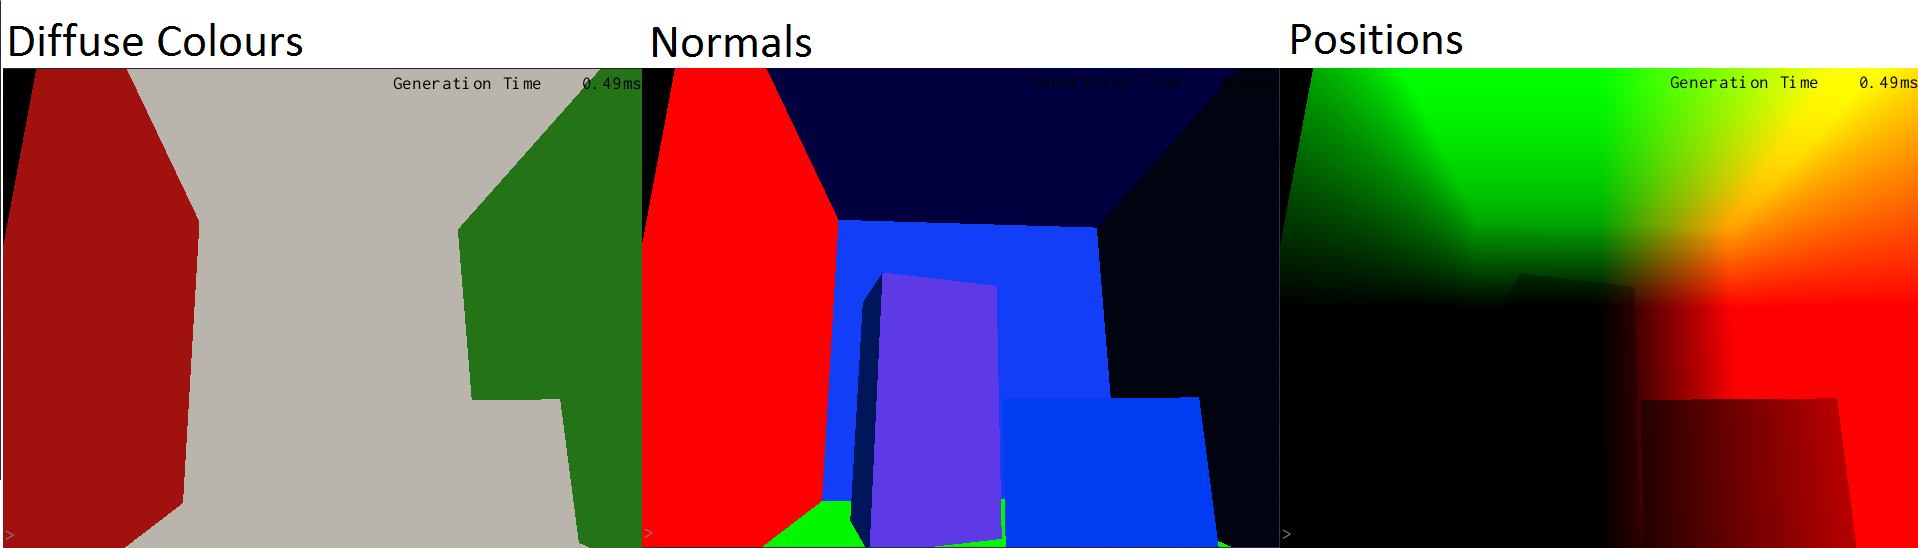
\includegraphics[width=1.0\textwidth]{img/def-rend/all}
    \caption{The contents of the G-buffer textures for the Cornell Box scene. There's no blue, since the eye direction is aligned along the negative Z-axis in view-space.}
    \label{fig-deferred}
\end{figure}

\subsubsection{Utilising the G-buffer}

When we have done the generation, we have a certain number of textures containing the geometric information for the scene on a per-fragment basis. We wish to use this data to do rendering calculations to produce our final scene. To do this we rasterise a single quad by an orthogonal projection, so that it fills the viewport exactly. In doing so, we have a 1:1 correspondence between our buffers and whatever target we're rendering to (be that another temporary offscreen buffer or the backbuffer.) We then sample data from whichever buffers we need to do our calculations, and use that data to calculate the desired shading. Listing \ref{list-deferred-use}, shows a deferred shader calculating lambertian lighting on a G-buffer.

\begin{lstlisting}[caption={Deferred Lambertian shader}\label{list-deferred-use},language=GLSL]
#version 330
in vec2 screenUV;

uniform sampler2D normals;
uniform sampler2D positions;
uniform sampler2D diff_colors;

uniform vec3 lPos;
uniform vec3 lInt;

out lambert;

main(void) {
	vec3 normal = normalize(texture(normals,screenUV));
	vec3 position = texture(position,screenUV);
	vec3 K_d = texture(diff_colors,screenUV);

	vec3 lV = normalize(lPos - position);
	
	lambert = K_d * lInt * dot(normal,lV);
}
\end{lstlisting}
To get the \verb?screenUV? vector we have a vertex attribute of 2 floats, that run between 0 and 1 along each axis.

If you ran this shader multiple times with additive blending enabled, every run would add a new light source to the render target, without needing to rerasterise the scene.

\subsubsection{Disadvantages}
While deferred rendering has its clear advantages in terms of running time, there are some things for which forward rendering has the edge. The primary one of these is the inability to do transparent materials. For instance, if the scene contained a refractive water layer, you'd be unable to write the normal data of this layer to the off-screen buffers, since it already has to contain the values for the materials under the water. A way to get around this is to do a forward render pass as the last step of the render pipeline, in which transparent objects are drawn with the uncleared depth buffer from the generation step. This would allow you to use the render target without the water (or other transparent surface) to look up offset values based on refraction index and normals of the surface.

Reflections can also cause problems, but they can be written directly to the G-buffer by the use of a stencil buffer and changes to the depth-test function. This, however, is only the case for G-buffers that do not have to be reconstructed from the depth buffer, whilst the method explained in \ref{section-reconstruction} has a few more caveats.

\subsection{The Deep G-buffer}
\label{section-deepbuffer}
When you start using the screen-space/G-buffer for more spatially conscious shading (such as radiosity or ambient occlusion,) pure single-layer G-buffers lack in apparent scene consistency. The traditional G-buffer simply does not contain anything beyond the top layer of geometry, and as such the same scene can seem visually inconsistent at two different angles. As an attempt to alleviate this shortcoming of deferred rendering, this thesis revolves around the use of a two layer deep G-buffer for global illumination approximations in screen-space. I will explain the technique as it is described in the paper \emph{Fast Global Illumination Approximations on Deep G-Buffers} by Michael Mara et al.\cite{deep-g-buffer}. What this method provides is a second layer of geometry, which means that shading stages has access to more geometric information about the scene, and thus is able to provide better and more visually consistent approximations of advanced effects.

The first thing we need to do to enable layered rendering, is to create array textures that contain the same number textures as the number of layers we wish to rasterise for our scene. Using array textures as render targets for an FBO works exactly like it does with with regular 2D textures, but obviously all texture have to have the same number of layers. The texture set up is also slightly different, since array textures are bound and initialised differently from flat textures in OpenGL. Listing \ref{list-deeptex} shows the OpenGL code to generate and initialise a 2-layer deep array texture.

\begin{lstlisting}[caption={Array texture initialisation for deferred rendering.}\label{list-deeptex},language=c++]
GLuint arrayTexture;

glGenTextures(1, &arrayTexture);
glBindTexture(GL_TEXTURE_2D_ARRAY,arrayTexture);

glTexParameteri(GL_TEXTURE_2D_ARRAY,GL_TEXTURE_MIN_FILTER,GL_NEAREST);
glTexParameteri(GL_TEXTURE_2D_ARRAY,GL_TEXTURE_MAG_FILTER,GL_NEAREST);
glTexParameteri(GL_TEXTURE_2D_ARRAY,GL_TEXTURE_WRAP_S,GL_CLAMP_TO_EDGE);
glTexParameteri(GL_TEXTURE_2D_ARRAY,GL_TEXTURE_WRAP_T,GL_CLAMP_TO_EDGE);

glTexImage3D(GL_TEXTURE_2D_ARRAY,0,GL_RGBA,width,height,2,0,GL_RGBA,GL_UNSIGNED_BYTE,0);
\end{lstlisting}

After we've tied our array textures to the FBO's colour attachments, we need to set up G-buffer generation such that it draws both layers of geometry to the texture. Figure \ref{fig-deep-buffer} shows the effect we wish to achieve, in which fragments that are occluded by the top layer of geometry are in stead written to the second layer of the G-buffer textures. In order to achieve this, we set up a geometry shader that emits all geometry directly and without modifications to both layers, as demonstrated in listing \ref{list-deepgeom}. Ultimately we do the test to determine whether or not to actually write the values in the fragment shader.

\begin{lstlisting}[caption={Geometry shader for 2-layer rendering.}\label{list-deepgeom},language=GLSL]
#version 330

layout(triangles) in;
layout(triangle_strip, max_vertices=6) out;

in vec3 outNormal[];
in vec4 outPos[];
in vec4 screenPos[];
in vec2 screenUV[];

out vec3 normalIn;
noperspective out vec2 screenUVFrag;
//noperspective because the screen UVs are linear in screen space.
out vec3 screenPosFrag;
flat out int layer;

void main() {
	layer = 0;
	gl_Layer = 0;
	for(int i = 0; i < 3; i++) {
		normalIn = outNormal[i];
		screenUVFrag = screenUV[i];
		screenPosFrag = vec3(screenPos[i]);
		EmitVertex();
	}
	EndPrimitive();
	
	layer = 1;
	gl_Layer = 1;
	for(int i = 0; i < 3; i++) {
		normalIn = outNormal[i];
		screenUVFrag = screenUV[i];
		screenPosFrag = vec3(screenPos[i]);
		gl_Position = outPos[i];
		EmitVertex();
	}
	EndPrimitive();
}
\end{lstlisting}

\begin{figure}[!ht]
  \centering
    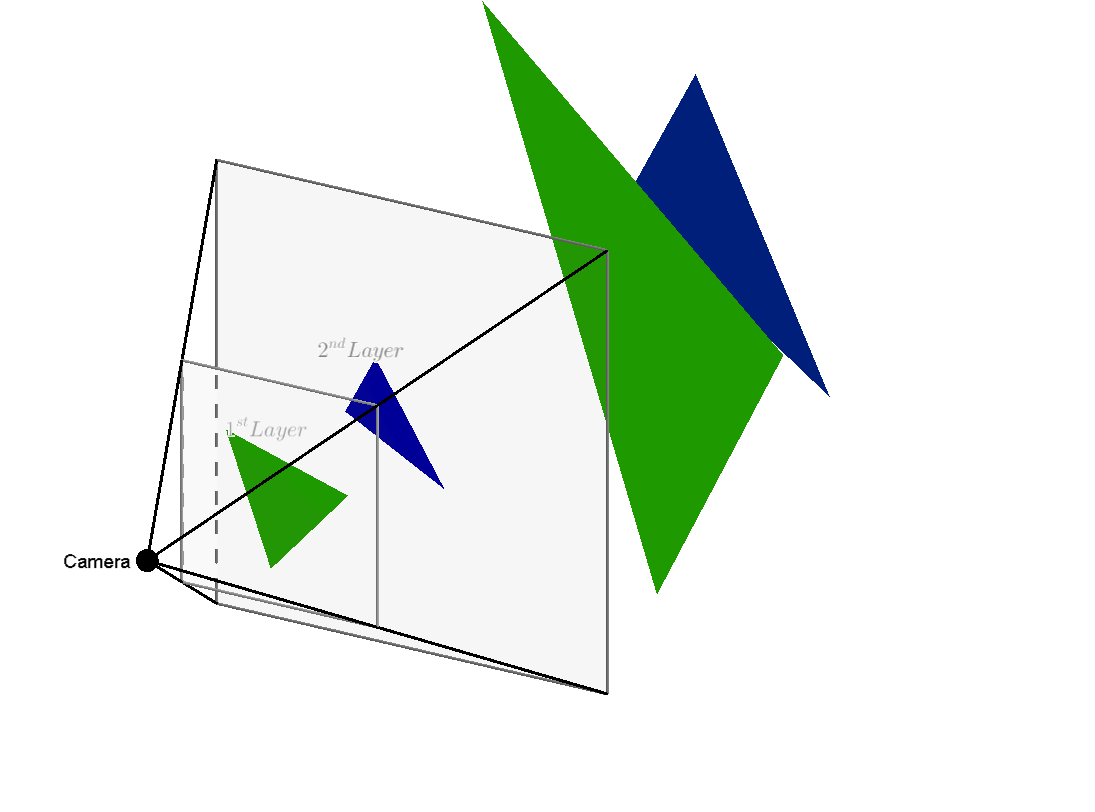
\includegraphics[width=0.8\textwidth]{img/2-layer}
    \caption{Illustration demonstrates the concept of a deep G-buffer. The green triangle is occluding the blue triangle. As a consequence, the blue one is written to the second layer of the G-buffer.}
    \label{fig-deep-buffer}
\end{figure}

Since the depth buffer is already making sure that the correct values are being written to the top layer of geometry, we can write values to layer 1 without doing any tests first. The second layer, however, is dependent upon whether or not geometry is occluded by the first layer. We can't use the currently bound depth-buffer to test this because it is actively being written to, and besides, there's no way of knowing what values might be written to it later (if we, for instance, determine that a piece of geometry does \emph{not} belong in the second layer, but another piece of geometry later overwrites it on the first layer.) As such, we need to buffer the depth buffer from the previous G-buffer generation, so that we can use it to predict whether or not a value belongs in the second layer. A naïve way to do this is to just use the previous run's depth buffer directly, and look up in its texture with the current run's screen UV-coordinates. This approach produces reasonable results, but at high generation times ($>20ms$) the secondary layer obviously "slags" when the camera moves around. This occurs because the shader is looking up "outdated" values. Another, more expensive option, is to rasterise geometry for both the current and previous frame, and use the previous frame's device coordinates to find the UVs to look up depth values. There's still some error related to the latter of the methods, but this is negligible compared to that of the former.

We also need to establish a minimal layer of separation between the two layers. Due to floating point imprecision, if we just look up the expected depth value of layer 1 and compare it to the Z value of the \verb=FragCoord=, we are going to Z-fighting artefacts in the second layer. The same effect causes shadow acne if you do not add a bias to a shadow map lookup. We set our separation in terms of fraction of the frustum depth. That is to say the space where 0 is the near-plane and 1 is the far-plane. This allows us to use the same layer of separation based on the definition of the projection planes. Choosing the right value to separate our two layers is a question of what parts of the scene we deem important. If we set it low enough, we can have back-facing geometry in the second layer, whereas high separation (or drawing with back-face culling) will cut off back-facing geometry to allow for deeper elements in the scene to appear in the second layer. Specifically how to set the value will vary depending on personal tastes and the scene you're working with. In this thesis we're working with a layer of separation that will draw back-facing geometry. To make the concept of depth consistent, we also linearise the depth values, since OpenGL packs depth values in a way that allows for more precision closer to the near-plane. To determine if a fragment is written to the second layer, we compare the calculated Z-coordinate with the Z-value read from the depth texture offset by our minimal layer of separation. If the calculated Z-coordinate is lower than the comparison value, we discard the fragment. The fragment shader for generating the 2-layer G-buffer can be seen in listing \ref{list-deepfrag}.

\begin{lstlisting}[caption={Fragment shader to generate the 2-layer G-buffer. No position is being written, which will be explained in section \ref{section-reconstruction}}\label{list-deepfrag},language=GLSL]
#version 330

in vec3 normalIn;
noperspective in vec2 screenUVFrag;
in vec3 screenPosFrag;
flat in int layer;

uniform sampler2DArray depth_texture;
uniform float near_plane;
uniform float far_plane;
uniform vec4 diff_color;
uniform vec4 spec_color;

layout(location=0) out vec3 normal;
layout(location=1) out vec4 diffColor;
layout(location=2) out vec4 specColor;

float linearDepth(in float depth){
	return (2.0 * near_plane) / (far_plane + near_plane - depth * (far_plane - near_plane));
}

void main() {

	switch(layer) {
		case 0:
			//Write data to buffer
			break;
		case 1:
			if(linearDepth(gl_FragCoord.z) <= linearDepth(texture(depth_texture,vec3(screenUVFrag,0)).r) + 0.01f)
				discard;
			else {
				//Write data to buffer
			}
			break;
	}

}
\end{lstlisting}

The comparison depth texture is a \verb=sampler2DArray= since it's 2-layered. We only use the first layer, however, since that is all we need to determine if a fragment belongs in layer if the output buffer. We also use \verb=sampler2DArray=s to sample when we do the deferred shading. Utilising the deep G-buffer is similar to the way we utilise a flat G-buffer, except our input textures are texture arrays. When we use it for our global illumination approximations we sample both layers at the same screen-space taps. If we wish to buffer information from a filter for both layers, we use a geometry shader to commit our full-screen quad twice, once for each layer.

\subsection{Scene Reconstruction}
\label{section-reconstruction}
The total memory cost of a naïvely implemented, 1-layer G-buffer with just normals, positions and material properties would, at the very least, be 128 bits, or 16 bytes, of information buffered per fragment. That is with 16-bit precision normals and positions ($16 bits * 3 channels * 2 buffers = 96 bits$, and a regular RGBA 8-bit precision diffuse reflectance (32 bits.) With 32-bit precision on positions, which would give noticeably better results, the total would end up being 176 bits, or 22 bytes, per fragment. For a 1080p (\verb=1920*1080=) buffer, the total memory usage for the G-buffer alone would end up at just under 44MB. Keep in mind that this is for the bare essentials, without any additional G-buffer related data like radiosity, SSAO, specular reflectance, shininess etc. It would definitely be possible to work around this memory usage by saving in other areas (textures, models;) even on a system with as little as 512MB of VRAM. Where the need to search for alternate solutions comes in, is with the use of a deep G-buffer. With a deep G-buffer all assumed VRAM useage for the G-buffer has to be multiplied by 2, meaning that our original 44MB becomes 87MB, and for every additional 32-bit buffer we use we have to add another 16MB (8MB for each layer.) Additionally, we need the previous frame's depth buffer to be able to tell whether or not a fragment belongs in the second layer of the G-buffer, which adds another 64 bits (8 bytes) per fragment (One for the current and one for the previous frame.) Luckily, there's a way to trade performance for less VRAM usage, both for positions and normals, by reconstructing information from the least amount of vital information. I will explain both of these here, but the product of this thesis only implements the reconstruction of positions.

\subsubsection{Reconstructing Positions}
In order to reconstruct positions, all we really need to buffer is the depth. In the reconstruction step, we can use the UV-coordinates of the full-screen quad to find the normalized device coordinates, and since we know the projection matrix by which the scene was projected, we can find the view-space coordinates of the fragment. Using the depth buffer also means we save a write operation when we generate the G-buffer, since we need a depth-buffer active for depth-testing regardless of whether or not we reserve its results for later. This offsets some of the cost of the reconstruction later. We tie a 2-layer array texture with internal format \verb=GL_DEPTH_COMPONENT32= to the depth attachment on the G-buffer generation FBO. The texture generation is the same as is shown in listing \ref{list-deeptex}, except the internal format is a 32-bit depth component. We then tie it to the depth attachment of the FBO like shown in listing \ref{list-depthFBO}. Note, that the depth attachment will have to be swapped around between frames due to its usage in predicting the contents of the deep layer.

\begin{lstlisting}[caption={Tying the depth texture to the depth component of the FBO}\label{list-depthFBO},language=c++]
GLuint FBO;
glGenFramebuffers(1,&FBO);
glBindFramebuffer(GL_DRAW_FRAMEBUFFER, FBO);
glFramebufferTexture(GL_DRAW_FRAMEBUFFER,GL_DEPTH_ATTACHMENT,depth_texture,0);
//Tie other textures to their relevant colour attachments.
\end{lstlisting}

With the depth information (as a number between 0 and 1) and screen-space UV-coordinates available in our reconstruction stage, we can find the normalised device coordinates for a fragment ($\mathbf{v} = 2((\mathbf{UV}_x,\mathbf{UV}_y,depth,0) - 0.5) + (0,0,0,1)$,) and using the inverse of the projection matrix used to project the scene in the generation stage, we can unproject these into coordinates with the right proportions in relation to each other, due to the following relationship:

$$\underline{\underline{M}}^{-1}\underline{\underline{M}} = \underline{\underline{I}}$$
$$\underline{\underline{M}}^{-1}\underline{\underline{M}} \mathbf{v} = \mathbf{v}$$
$$\underline{\underline{P}}^{-1}\underline{\underline{P}}\underline{\underline{V}}\underline{\underline{M}}\mathbf{v} = \underline{\underline{V}}\underline{\underline{M}}\mathbf{v}$$

To get the true view-space coordinates we ultimately do W-division: $\mathbf{X} = \frac{\mathbf{v}_{xyz}}{\mathbf{v}_w}$. In doing this, we save 64 bits per layer per fragment, or a total of 128 bits of storage per fragment for positions, assuming a 96-bit position buffer. We also save at least two memory taps, due to the GPU needing more memory reads to retrieve a 96-bit texel than a 32-bit one.

A major disadvantage with reconstructing the scene from a depth-buffer, is that we can no longer do reflections using deferred rendering. This is because the view matrix is different for parts of the scene that are reflected, and as such the entire depth buffer cannot be reconstructed in a single go. This can be fixed, however, by either doing ray-traced reflections in screen-space in a later filtering stage or using stencil buffers to which you draw the reflective parts of the scene to only reconstruct and shade parts of the scene for which a given MVP-matrix is valid. This method does add overhead both in terms of more state changes, more shading computations and more memory usage.

\subsubsection{Reconstructing Normals}
In regards to normals, we can utilise the fact that we know its length in order to reconstruct the third of its coordinates from the two others by simply doing $\pm Z = \sqrt{X^2 + Y^2 - 1}$. While this in and of itself is not very complicated, and most modern GPUs do the calculation $\frac{1}{\sqrt{X}}$ in a single cycle, meaning it wouldn't necessarily be very expensive, the issue arises in determining the sign of the third coordinate. Since central projection, which is what I use in the product of this thesis, allows for geometry facing away from the near plane to be rasterised, and X and Y coordinates are independent of screen-space positions, we would need to somehow buffer the sign of Z if we wanted to save only two coordinates for every normal. One way to do this would be to use an available 8-bit channel in one of the colour buffers, which both have an alpha channel available (although we use the $\rho_s$ alpha to store shininess.) This, however, requires us to do an additional texture tap whenever we want to use our normals. A better solution would be to sacrifice precision in either the Y or X coordinate by encoding the sign of Z into the least significant bit of the mantissa of either. The problem with this method is that it requires the use of integer operations, which are not widely supported by GPUs yet, and there's some performance hit involved in doing so.
I originally used \verb$R11_G11_B10$ float textures to buffer normals, which does not have a sign on its mantissa. These were encoded by dividing by 2 and adding a half. However, the lack of precision in this format (causing inconsistent lighting between angle changes,) and the hardware related costs of interpreting them for use in a shader meant that I ultimately settled on the traditional \verb$RGB16F$ format.

\section{Omnidirectional Shadowmapping}
While we we assume for radiosity that the visibility term is equal to 1, and aren't doing any occlusion testing on the hemisphere samples, we wish to do occlusion testing for the diffuse reflectance of radiance directly from the light source. We will use a simple Lambertian shader for our initial radiosity result, multiplied by a visibility term, which we will find based on a look up into a shadow map. Lambertian shading calculated diffuse radiance from a surface like so:

$$L_e(\mathbf{x}) = \frac{1}{atten}\frac{\rho_d}{\pi} I_l cos(\theta) V(\mathbf{l} \rightarrow \mathbf{x})$$

Where $atten$ is the attenuation of the light (for directional lights this is 1,) $\rho_d$ is the diffuse reflectance, which is a vector with values between 0 and 1, $I_l$ is the intensity of the light source, $\theta$ is the angle between the normalised vector from our point to the light source and $V()$ is the visibility term.

In order to evaluate the visibility term we will employ a shadow-map. However, since we want to support point lights and work regardless of what and how many elements are in the scene, this is slightly more tricky than simply implementing a simple one-texture shadow-map that contains normalized clip-space coordinates. To accomplish full coverage around our point light, we need to use something called an omni-directional shadow map. There are several ways to achieve this, but the simplest and most precise is one in which you render your scene unto a cube-map and buffer the clip-space distance from the light source to a given fragment. The process of rendering to a cube map is very similar to that of rendering the deep G-buffer, in that the cube-map is essentially just a 6-layered array texture in which each layer represents a face on the cube. The process of preparing a cube map as a render target is demonstrated in listing \ref{list-cube-tex}. Notice, we only tie a render target to the depth buffer, since that is all we need.

\begin{lstlisting}[caption={Setting up the cube map for rendering}\label{list-cube-tex},language=c++]
//Texture and FBO generation
glGenTextures(1, &shadowDepth);
glGenFramebuffers(1, &shadowFBO);

glBindTexture(GL_TEXTURE_CUBE_MAP, shadowDepth);
//Set parameters for texture
glTexParameteri(GL_TEXTURE_CUBE_MAP, GL_TEXTURE_WRAP_S, GL_CLAMP_TO_EDGE);
glTexParameteri(GL_TEXTURE_CUBE_MAP, GL_TEXTURE_WRAP_T, GL_CLAMP_TO_EDGE);
glTexParameteri(GL_TEXTURE_CUBE_MAP, GL_TEXTURE_WRAP_R, GL_CLAMP_TO_EDGE);
glTexParameteri(GL_TEXTURE_CUBE_MAP, GL_TEXTURE_MAG_FILTER, GL_LINEAR);
glTexParameteri(GL_TEXTURE_CUBE_MAP, GL_TEXTURE_MIN_FILTER, GL_LINEAR);
//For each layer in the cube-map we initialise its contents
for(GLuint i = 0; i < 6; i++) {
	glTexImage2D(GL_TEXTURE_CUBE_MAP_POSITIVE_X + i, 0, GL_DEPTH_COMPONENT32F, SHADOW_WIDTH, SHADOW_HEIGHT, 0, GL_DEPTH_COMPONENT, GL_UNSIGNED_BYTE, nullptr);
	
glBindFramebuffer(GL_DRAW_FRAMEBUFFER,shadowFBO);
//Tie the cube map texture to the depth attachment of the FBO.
glFramebufferTexture(GL_DRAW_FRAMEBUFFER,GL_DEPTH_ATTACHMENT,shadowDepth,0);
\end{lstlisting}

We use the same projection matrix for all layers, which is a central projection with a $\frac{\pi}{2}$ field of view. The FOV has to be exactly that, since that means the frustums for all sides of the cube line up such that when geometry is split between two sides, it will line up on the cube. We also set the view matrices such that they line up in accordance with \cite{cubetex}. We then draw the length of the position vector divided by the far plane to the depth buffer. An important note here is to \emph{not} let the pipeline interpolate the depth between vertices, but calculate it in the vertex shader based on the interpolated position vector, since the depth does not change linearly across an edge. We use the length of the position vector since it easens our look-up when we evaluate the visibility term. The length of the vector from a point to the light source can then be used to determine occlusion. If we used the projected fragment depth, we'd first have to figure out which coordinate of the light vector to use for our comparison.

Since the view matrices used to generate the shadow map are in world space, and we calculate data to be in screen-space, when we do the lighting calculations we have to also remember to multiply our regenerated position vector by the inverse view matrix originally used to rasterise the scene. This way we obtain world-coordinates, which are needed for the shadow map look up.

One of the major advantages of using a cubemap texture for our omni-directional shadowmap is that you access cubemaps by looking up a direction in stead of a UV-coordinate. What this means is that we can use the world-space normalized light vector to find the value we need to compare by to determine visibility. We then simply take the length of the light vector, divide it by the far plane, and if it is less than or equal to the value in the shadowmap, the fragment is \emph{not} occluded. We subtract a very small bias from the light vector length to get rid of shadow acne.

\section{Radiosity}
\label{section-radiosity}
Radiosity is a method to determine light transfer between purely diffuse surfaces. That is to say it covers only the case in which incident radiance at a surface is distributed equally in all directions, and the amount of energy that is transferred between surfaces by this method. We will take a point of departure in the rendering equation, explain the predominant "slow" radiosity method of dividing the scene into patches and explain the screen-space approximation used in the final product.

\subsection{The Rendering Equation}
\label{section-renderingequation}
The rendering equation sets up the radiance from a point towards another point as the sum of its emitted radiance and an integral over the hemisphere to gather radiant exitance based on incident radiance, outgoing direction, incoming direction and the wavelength of light. It can be denoted in multiple ways, here we will write it like this: Figure \ref{fig-rendering-eq} denotes what symbols represent spatially.

$$L(\mathbf{x} \rightarrow \overline{\omega_0},\lambda) = L_e(x \rightarrow \omega_o,\lambda) + \int_\Omega F_r(\mathbf{x},\overline{\omega_i},\overline{\omega_0},\lambda) I_i(\omega_i \rightarrow \mathbf{x}) \cos(\theta) d\omega_i$$

\begin{figure}[!ht]
  \centering
    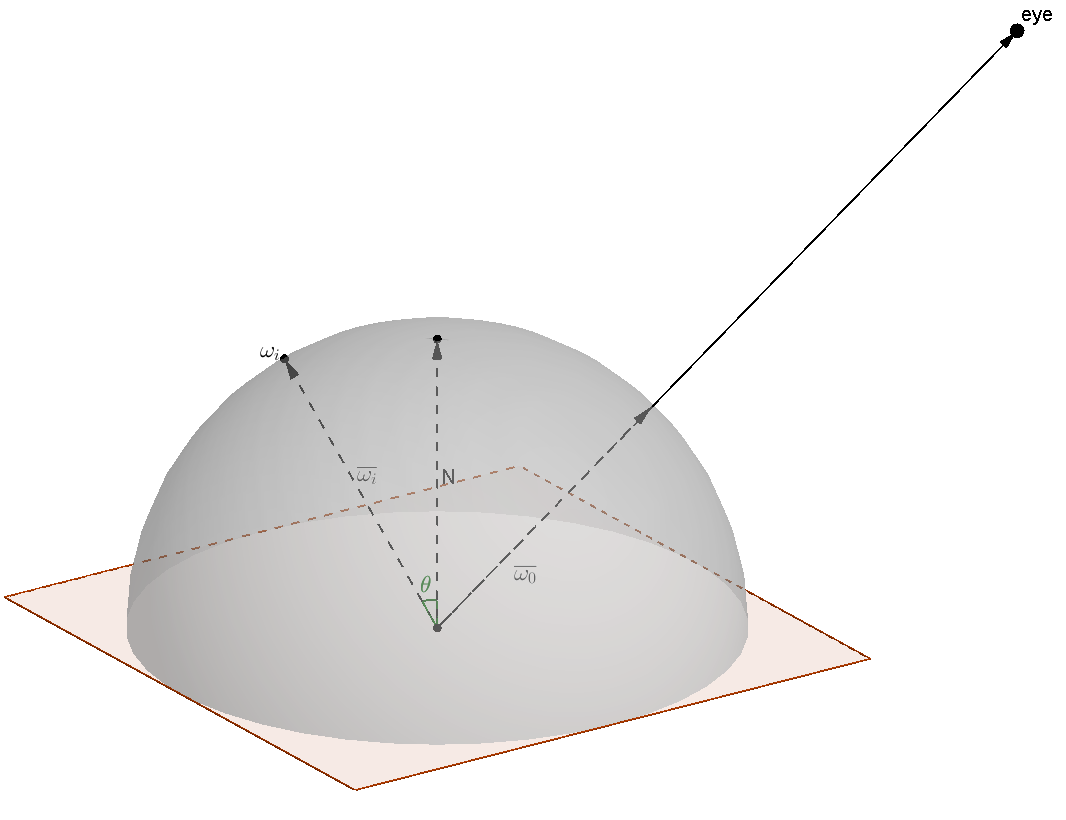
\includegraphics[width=0.8\textwidth]{img/rendering-eq}
    \caption{A visual representation of the rendering equation, with symbolic values annotated.}
    \label{fig-rendering-eq}
\end{figure}

We integrate over the hemisphere around the normal of the point, to gather radiance reflected towards our view position.\\
$\mathbf{x}$ represents the point in space we're currently investigating.\\
$\overline{\omega_0}$ is the normalized vector from $\mathbf{x}$ towards the point to which radiance is emitted (or the view point.)\\
$\lambda$ is the wavelength of the light.\\
$\Omega$ is the surface of the hemisphere.\\
$\omega_i$ refers to the infinitessimal solid angle on the hemisphere.
$\overline{\omega_i}$ is the direction from $\mathbf{x}$ to $\omega_i$.\\
$\theta$ is the angle between the normal of $\mathbf{x}$ and $\overline{\omega_i}$\\

$L_e()$ is emitted radiance, which is not part of the scope of this thesis. For the purpose of radiosity, the interesting part is the integral. One way to think of it is that it's an integral of a function $I(\omega)$ whose function values are the irradiance incoming from are $\omega$ which runs over a known surface (the hemisphere.) $F_r$ is the Bi-Ray Distribution Function, which is a function that varies depending on the material properties of the point of incidence. It produces a factor by which to multiply the irradiance from $\omega_i$, $I_i$, based on $\overline{\omega_i}$, $\overline{\omega_0}$ and $\lambda$. Like mentioned radiosity is only concerned with the case of perfectly diffuse surfaces, meaning that total irradiance is distributed equally across the hemisphere, regardless of incoming direction. As such, the BRDF is completely independent of the direction of irradiance (as long as it is on the hemisphere) and how it relates to the view direction. It is, however, dependent upon $\lambda$, since the material will absorb light of certain wavelengths based on its colour. The BRDF of a perfectly diffuse surface is therefore simply $K_d$ or $\frac{\rho_d}{\pi}$.

For diffuse light transfer we will assume a perfectly closed system, in which all surfaces are perfectly diffuse. This will allow us to write up a rendering equation for radiosity:

$$L(\mathbf{\mathbf{X}} \rightarrow \mathbf{e}) = B(\mathbf{X}) = \int_\Omega \frac{\rho_d}{\pi} B(\mathbf{Y}) \cos(\theta) d\omega_i$$

What this means is that radiance received for our eye point, $\mathbf{e}$, from point $\mathbf{X}$, is obtained by integrating radiosities for all points visible from point $\mathbf{X}$ across the hemisphere.. Point $\mathbf{Y}$ denotes the point in direction $\overline{\omega_i}$ from $\mathbf{X}$. A simple way to obtain multiple bounces from a naive implementation of this equation, would be to consider it a recursive function. That is to say, for every $\omega_i$, consider its corresponding $\mathbf{Y}$ the subject of another radiosity gather, in which the eye point, $\mathbf{e}$ is now the original $\mathbf{X}$ and $\mathbf{X}$ is now the original $\mathbf{Y}$. For every layer of recursion added to this method, we'd get another bounce. However, running such an algorithm for every pixel in a ray tracer would be prohibitively expensive, even with decent sampling optimisations. The complexity of such a recursive method would be $O(p \cdot b^n)$, where $p$ is the total number of pixels sampled, $b$ is the number of bounces and $m$ is the number of samples used to approximate the integral. As such, other methods are employed to approximate this effect in a more reasonable time.

\subsection{The Patch Method}
The patch method is the most common way to solve the radiosity problem in "slow" time (as opposed to real-time.) In it, you divide your scene into discrete patches, each of which has an amount of energy attached to it, which is distributed as radiosity to other patches in the scene. It is usually used as a pre-baking method, in which radiosity is done for diffuse surfaces and mapped unto the scene when it is ray-traced, or, for real-time applications, rasterised. It has the distinct disadvantage for the latter application, since the generation time does not allow for the radiosity map to be regenerated on-the-fly (at least not on current generation hardware.) Therefore radiosity by the patch method will typically be done only once for real-time applications, which means that radiosity for scenes with dynamic lighting, shadows and geometry will not change over time. The product of this thesis does not implement a patch method, but as was mentioned it is the most common method employed, and will provide a good contrast to the screen-space method explained in \ref{section-ssradiosity}.

With the patch method, we wish to approximate the integral over the hemisphere with discrete patches in space. A discretisation of the radiosity equation from \ref{section-renderingequation}, in which we loop over all other patches in the scene, to gather up all radiosity for a single patch, looks like this:

$$B(X) = \sum_{i=0}^{n} \frac{\rho_d}{\pi} \int_{t_0} \int_{t_i} B(i) \cos(\theta_i) V(x \rightarrow y) dt_i dt_0$$
$n$ is the number of patches in the scene.\\
$t_0$ is the patch for which we are currently gathering radiosity.\\
$t_i$ is the $i^{th}$ patch.\\
$V()$ is the visibility term, which is either a value of 1 or 0 depending on whether or not the infinitesimal point $y$ on $t_i$ is visible from the infinitesimal point $x$ on $t_0$.

We integrate over our patch, and for every infinitesimal point on it, we integrate over the patch from which we are currently gathering radiosity. Of course, these internal integrals are still not discretised, but to achieve simple computations we replace them with something called the form factor. What we essentially want is to determine the area which $t_i$ covers on the hemisphere of $t_0$. We also include $cos(\theta_i) V(x \rightarrow y)$ in this factor, so that all the geometry terms are included. We rewrite $cos(\theta_i) V(x \rightarrow y)dt_i dt_0$ to:\cite{radiosity}

$$F_{0i} = \frac{1}{A_0} \int_{A_0} \int_{A_i} \frac{cos(\theta_i) cos(\theta_0)}{\pi r^2}  V(x \rightarrow y) dA_i dA_0$$

Where $r$ is the distance from $t_0$ to $t_i$. We estimate this numerically by simply replacing $dA_i d_A0$ by the areas of the two patches ($A_i$ is eliminated because of the division):

$$F_{0i} \approx A_i \frac{cos(\theta_i) cos(\theta_0)}{\pi r^2}  V(x \rightarrow y)$$

The equation is currently written from the point of view of the gatherer; that is to say we calculate radiosity received based on an integral over the hemisphere of the gatherer. For the patch method it makes more sense to consider the point of the view of the distributor, seeing as once the distributor's energy has been exhausted, we can set its total energy to zero, since it has all been expended. Making such a change is fairly straight forward in code, seeing as the form factor and visibility terms merely have to be swapped around. If we consider $\mathbf{X}$ our distributor, we loop over all other patches, and based on the form factor, visibility term and radiosity of $\mathbf{X}$, we add to the radiosity of these patches. This type of buffered method does not allow us to do multiple bounces sequentially, as the distribution changes the radiosity levels of other patches. However, we can always make sure to distribute for the most significant patch at any given time, by sorting the list of patches by highest radiosity. Listing \ref{list-patchDist} shows how a single patch distributes its energy.

\begin{lstlisting}[caption={A single patch distributing its energy to other patches in the scene.}\label{list-patchDist},language=c++]
List<Patch*> patches;
Patch currentPatch = pathces[0];
for(int i = 1; i < patches.length; i++) {
    patches[i]->radiosity += patches[i]->K_d * currentPatch->radiosity
    * max(dot(currentPatch->normal,normalize(pathces[i]->pos - currentPatch->pos)),0);
    * visFactor(currentPatch,&patches[i])
    * formFactor(currentPatch,&patches[i]);
}
currentPatch.radiosity = 0;
\end{lstlisting}

There are multiple ways to evaluate the visibility factor. One is to trace a ray through the scene along the vector between the two patches and test for collisions. Another one, which also easens the evaluation of the form factor, is to project other patches unto a cube around the distributor patch using a rasteriser pipeline with depth testing (aka the hemicube method.)

\subsection{Screen-Space Methodology}
\label{section-ssradiosity}
The method we wish to deploy is one that takes advantage of the deep G-buffer specified in \ref{section-deepbuffer} to do real-time radiosity calculations. As such, we need a screen-space approximation. In this section I will explain a way to achieve such an approximation by sampling both layers of the G-buffer according to a parametrised curve using quasi-Monte Carlo sampling, and how to consider the rendering equation for radiosity to approximate the integral over the hemisphere.

\subsubsection{Monte Carlo Integration}
Monte Carlo sampling is a way to approximate integrals by doing random samples from the total of function values. In order to explain it, we will take a point of departure in Riemann Integration. The idea behind the Riemann Integral is that in order to find the integral of a given function, you sum up the function values of incrementing $x$-values and multiplying by the change in $x$.

$$\mathbf{F}(x) = \sum_{i = 0}^{n}f(x\frac{i}{n}) \Delta x$$

Where $n$ is the number of $x$-values used to find the integral and $\Delta x$ is the width of each segment, or $\frac{x}{n}$. If we let $n$ tend towards $\infty$ we get a continuous integral.

For our purposes, however, we do not know a function describing the distribution of irradiance on the hemisphere, but we are able to sample our screen-space for function values. Monte Carlo integration is a way to find the integral of an unknown function, by sampling function values at random, and giving them all equal weight. In a sense, it is a return to the base of the Riemann Integral. We wish to use Monte Carlo integration to solve the following integral:

$$L(\mathbf{X} \rightarrow \mathbf{e}) = B(\mathbf{X}) = \int_\Omega \frac{\rho_d}{\pi} B(\mathbf{Y}) \cos(\theta) d\omega_i$$

Ideally, to approximate this integral we would trace rays in cosine-weighted random directions around the normal of $\mathbf{X}$, and weigh each of them based on their proportion of the hemisphere. We write up the summation like so:

$$B(\mathbf{X}) = \sum_{i=0}^{n} \frac{\rho_d}{\pi} B(\mathbf{Y}(\omega_i)) \cos(\theta) \Delta \omega_i$$

Here $\omega$ can be considered an array of length $n$ of properly distributed, random directions. The point $\mathbf{Y(\omega_i})$ is the point resulting from ray-tracing in direction $\omega_i$. If we let the size of the array, $n$, tend towards infinity, the result becomes accurate thanks to the Law of Large Numbers. Since we know that the total area of the hemisphere is $2\pi$, the sum of all infinitesimal angles, $d\omega_i$, is $2\pi$, and we assume that for every ray we trace, the result we get from the scene will cover an equal part of the hemisphere, we get the following sum:

$$B(\mathbf{X}) = \frac{2\pi}{n} \frac{\rho_d}{\pi} \sum_{i=0}^{n} B(\mathbf{Y}[\omega_i]) \cos(\theta)$$

Of course, a problem occurs since we're working in screen-space, and that is that we do not have access to a ray-tracer, and only geometry in the viewing frustum is immediately available to us. The former will be alleviated by the use of a Quasi-Monte Carlo sampling method explained in the next section. The latter is an inherent problem with screen-space methods, and while remedies exist in the form of other non-screen-space methods, this problem will not be solved as part of this thesis.

\subsubsection{Quasi-Monte Carlo}
Since Monte Carlo approximations rely on completely random samples of function values, with a low number of samples the relative chance of errors is high. This occurs because true randomisation (or even pseudo-randomisation) only guarantees tendency towards the result for a high number of samples (The Law of Large Numbers.) For real-time applications we're only going to have time for a limited number of texture taps per pixel per frame drawn. As such, we need a sampling strategy that distributes our chosen sampling points to cover as much space as possible, while also maintaining some randomisation to avoid structural bias. Thus, we want a function to distribute our sample point evenly in screen-space around our gather point under the assumption that this will give us the most even distribution of points on our hemisphere. We also want it to be distributed around the point for which we are gathering, which means we are looking for something to offset our sample taps.

To achieve these goals we will use a tap pattern that runs along a parametrised spiral, with every tap spaced evenly out along the spiral. We will start by looking at the parametrisation of a spiral, and how the different parameters for it affect its form. The parametric curve of a spiral in its simplest form is defined as:

$$\mathbf{v}(t) = t \begin{pmatrix}\cos(t) \\ \sin(t) \end{pmatrix}$$

While the curve for this function will produce a spiral, it doesn't allow much control of its form, and the arms of the spiral will be increasingly distant for larger values of $t$. We want fairly evenly distributed points in screen-space, with a way to randomise our spiral, control its radius and the number of turns it does within this radius. To do this we employ the following parametrisation:\cite{deep-g-buffer}

$$\sigma = t + \frac{\psi}{tau} $$
$$\theta = 2\pi\sigma\tau + \phi $$
$$\overline{u} = \begin{pmatrix}\cos(\theta) \\ \sin(\theta) \end{pmatrix} $$
$$h = R \sigma $$
$$\mathbf{v} = h \overline{u}$$
$$0 < t < 1, 0 < \phi < 2\pi, 0 < \psi < 1$$

This gives us a number of parameters to work with. $R$ is the radius of our spiral, when $t$ is 1, the length of $\mathbf{v}=R$. $\tau$ is the number of spiral turns are inside the spiral before it reaches $t = 1$, $\phi$ and $\psi$ are used to allow for some randomisation of the spiral; $\phi$ is an angle by which we rotate the entire spiral (randomising this to be unique for each fragment will allow us to trade structural noise for more random noise.) $\psi$ allows us to offset the start of the spiral up to one turn. Figure \ref{fig-spiralparam} demonstrates the spiral and how the parameters change its form.

\begin{figure}[!ht]
\begin{tabular} {| l | c | c | c | c |}
\hline
& 
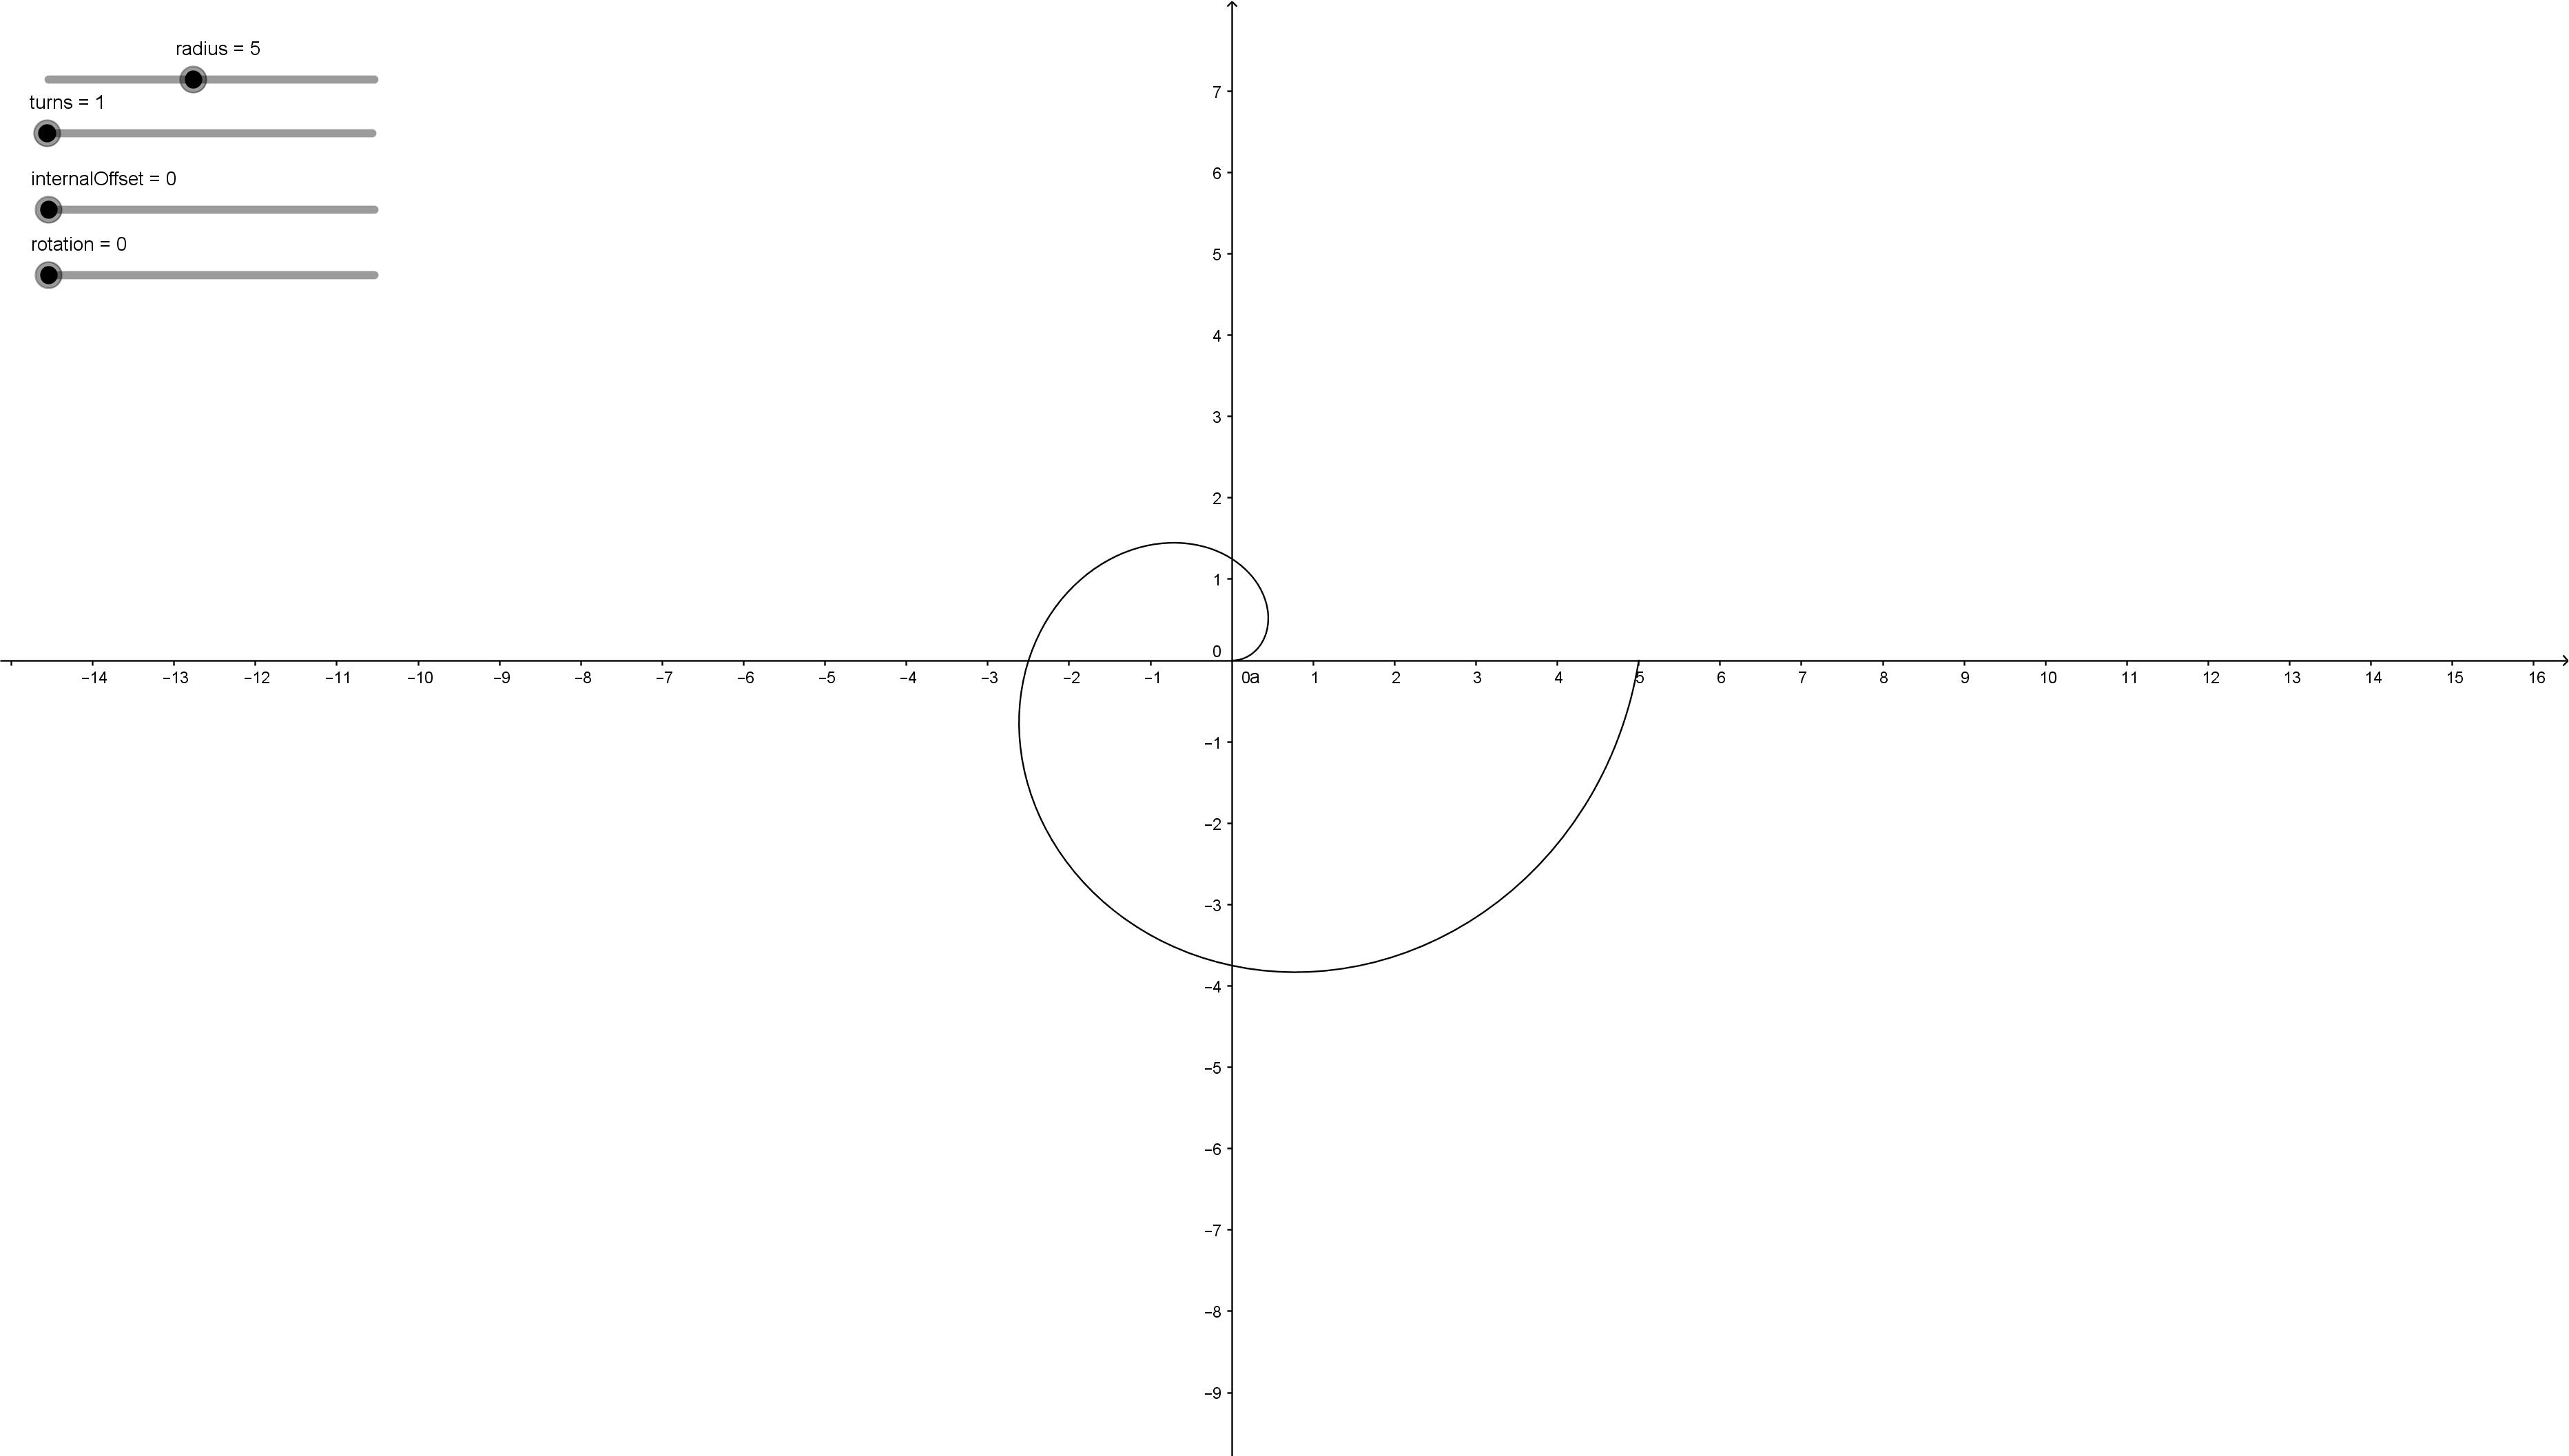
\includegraphics[scale=0.2,trim={10cm 4.65cm 11.3cm 3.0cm},clip]{img/spiral/1turn}
&
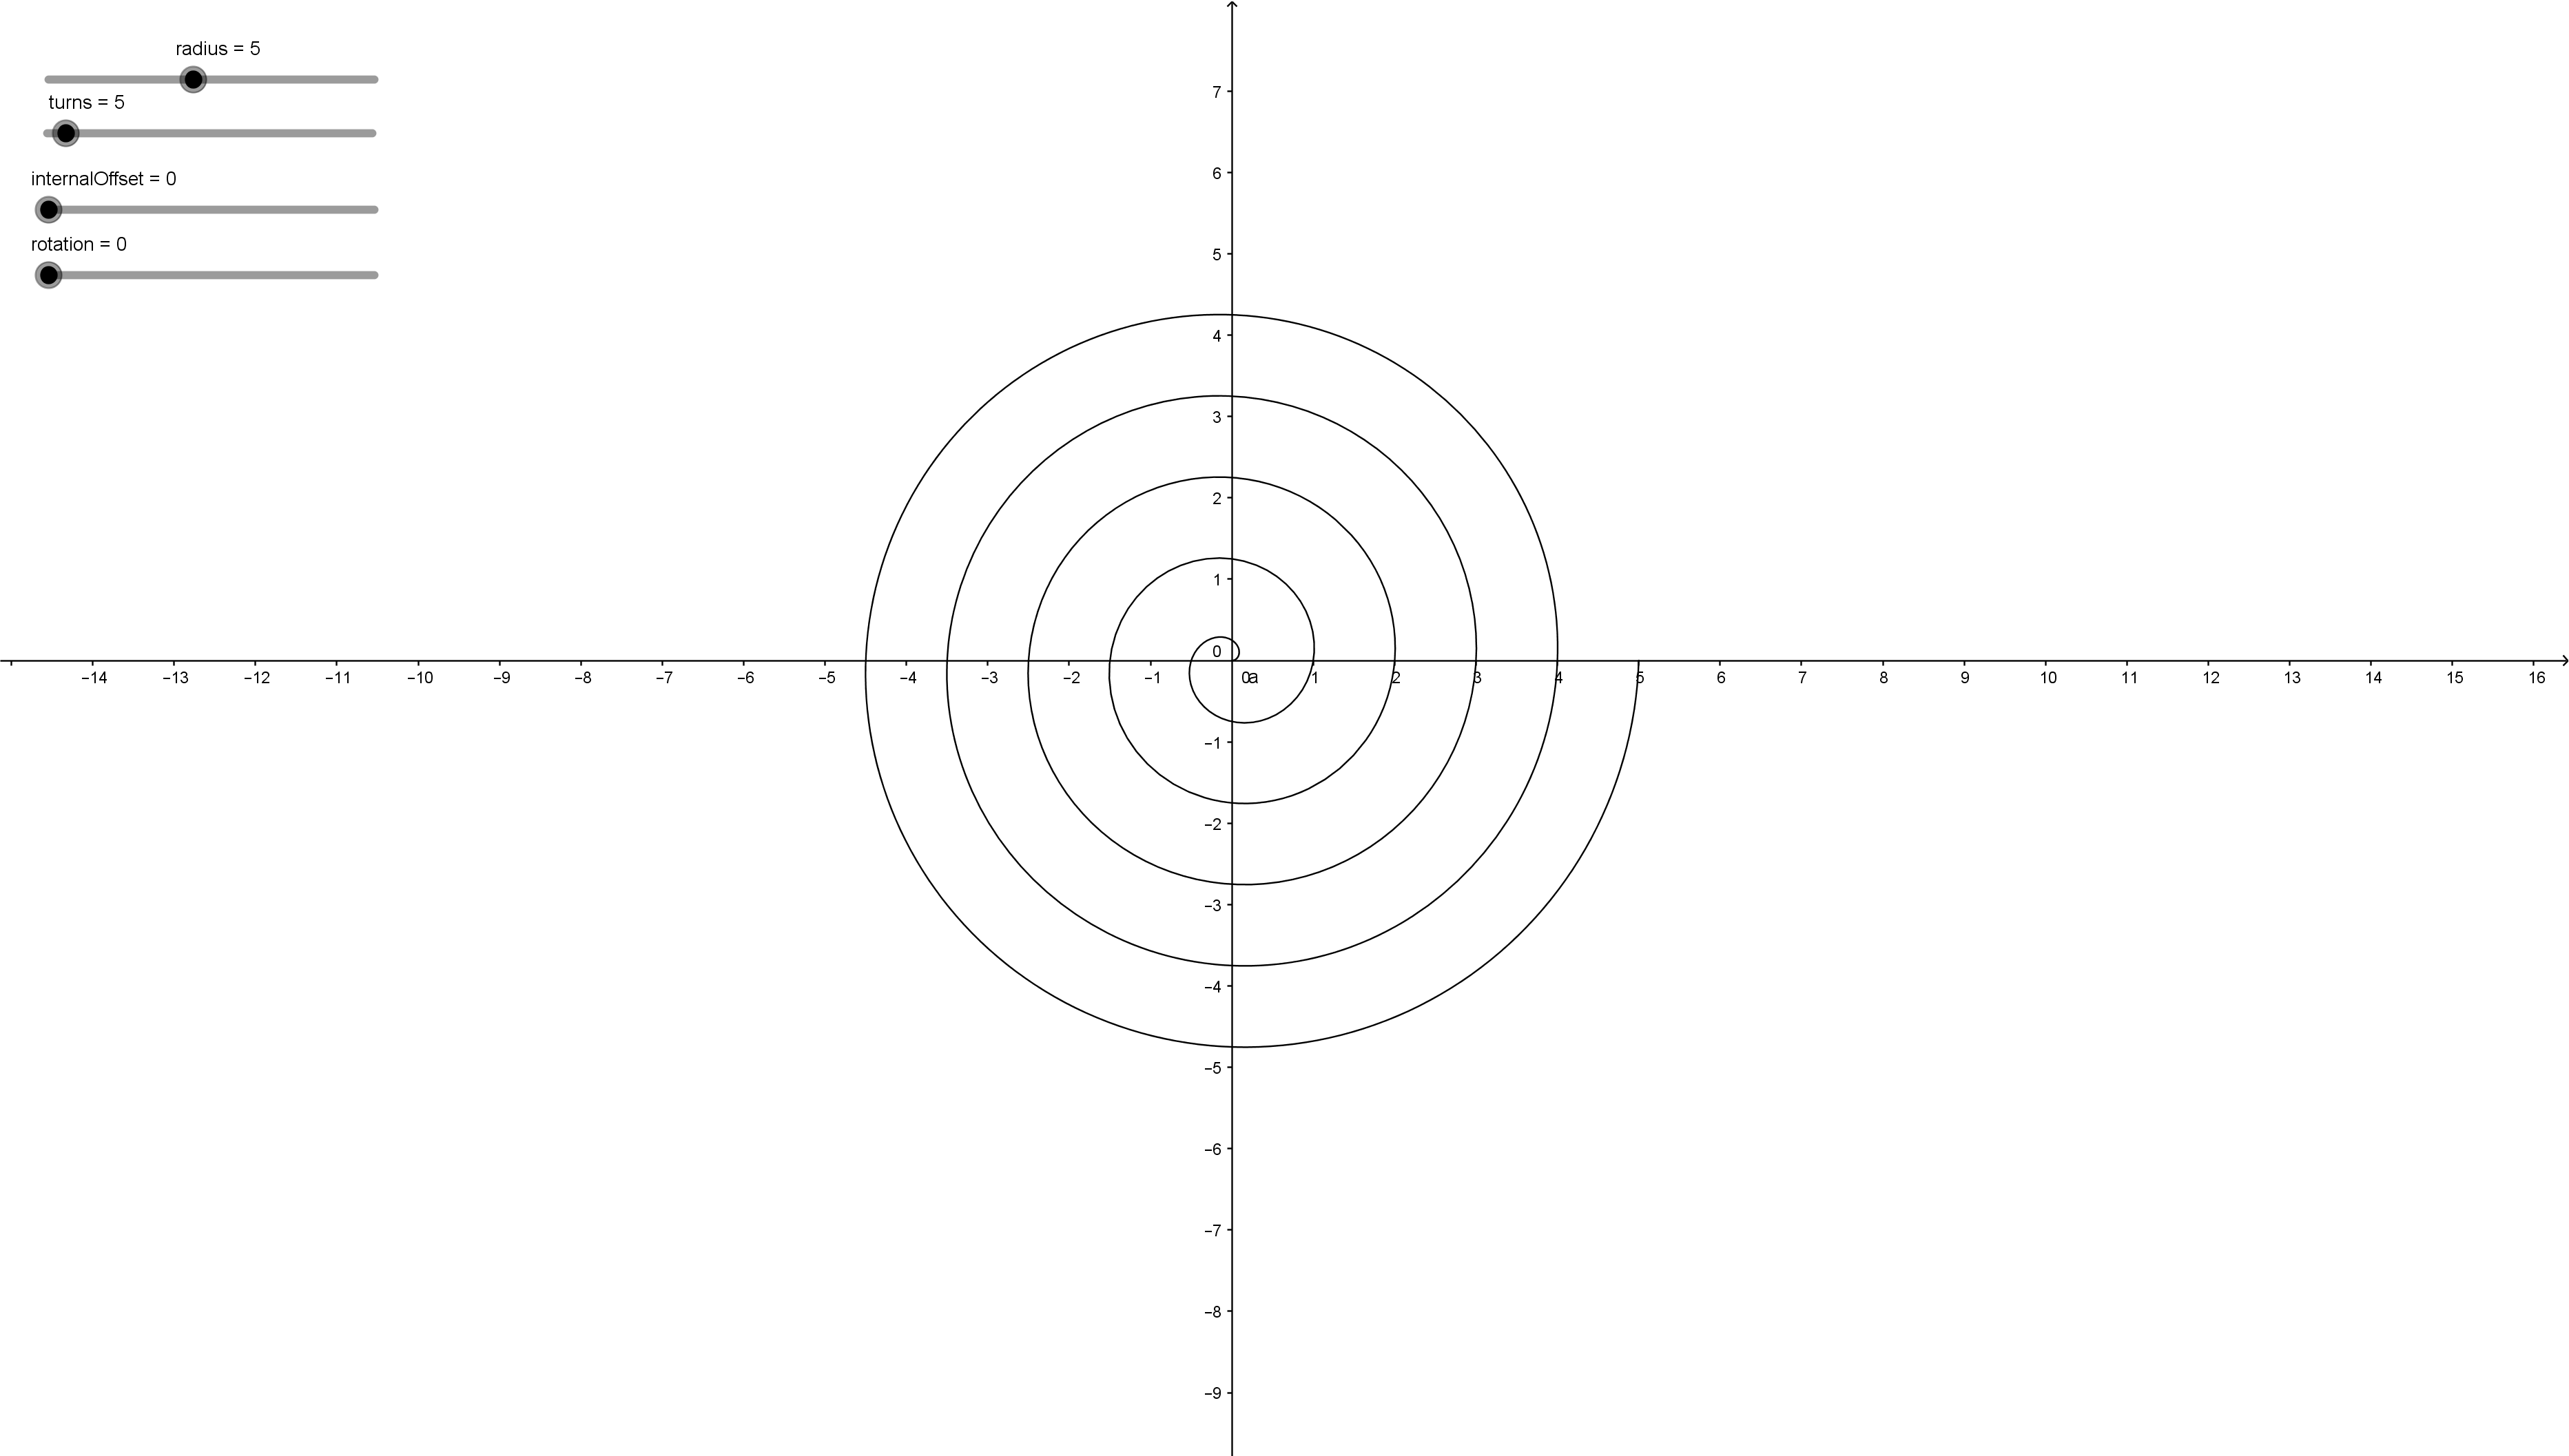
\includegraphics[scale=0.2,trim={10cm 4.65cm 11.3cm 3.0cm},clip]{img/spiral/5turns}
&
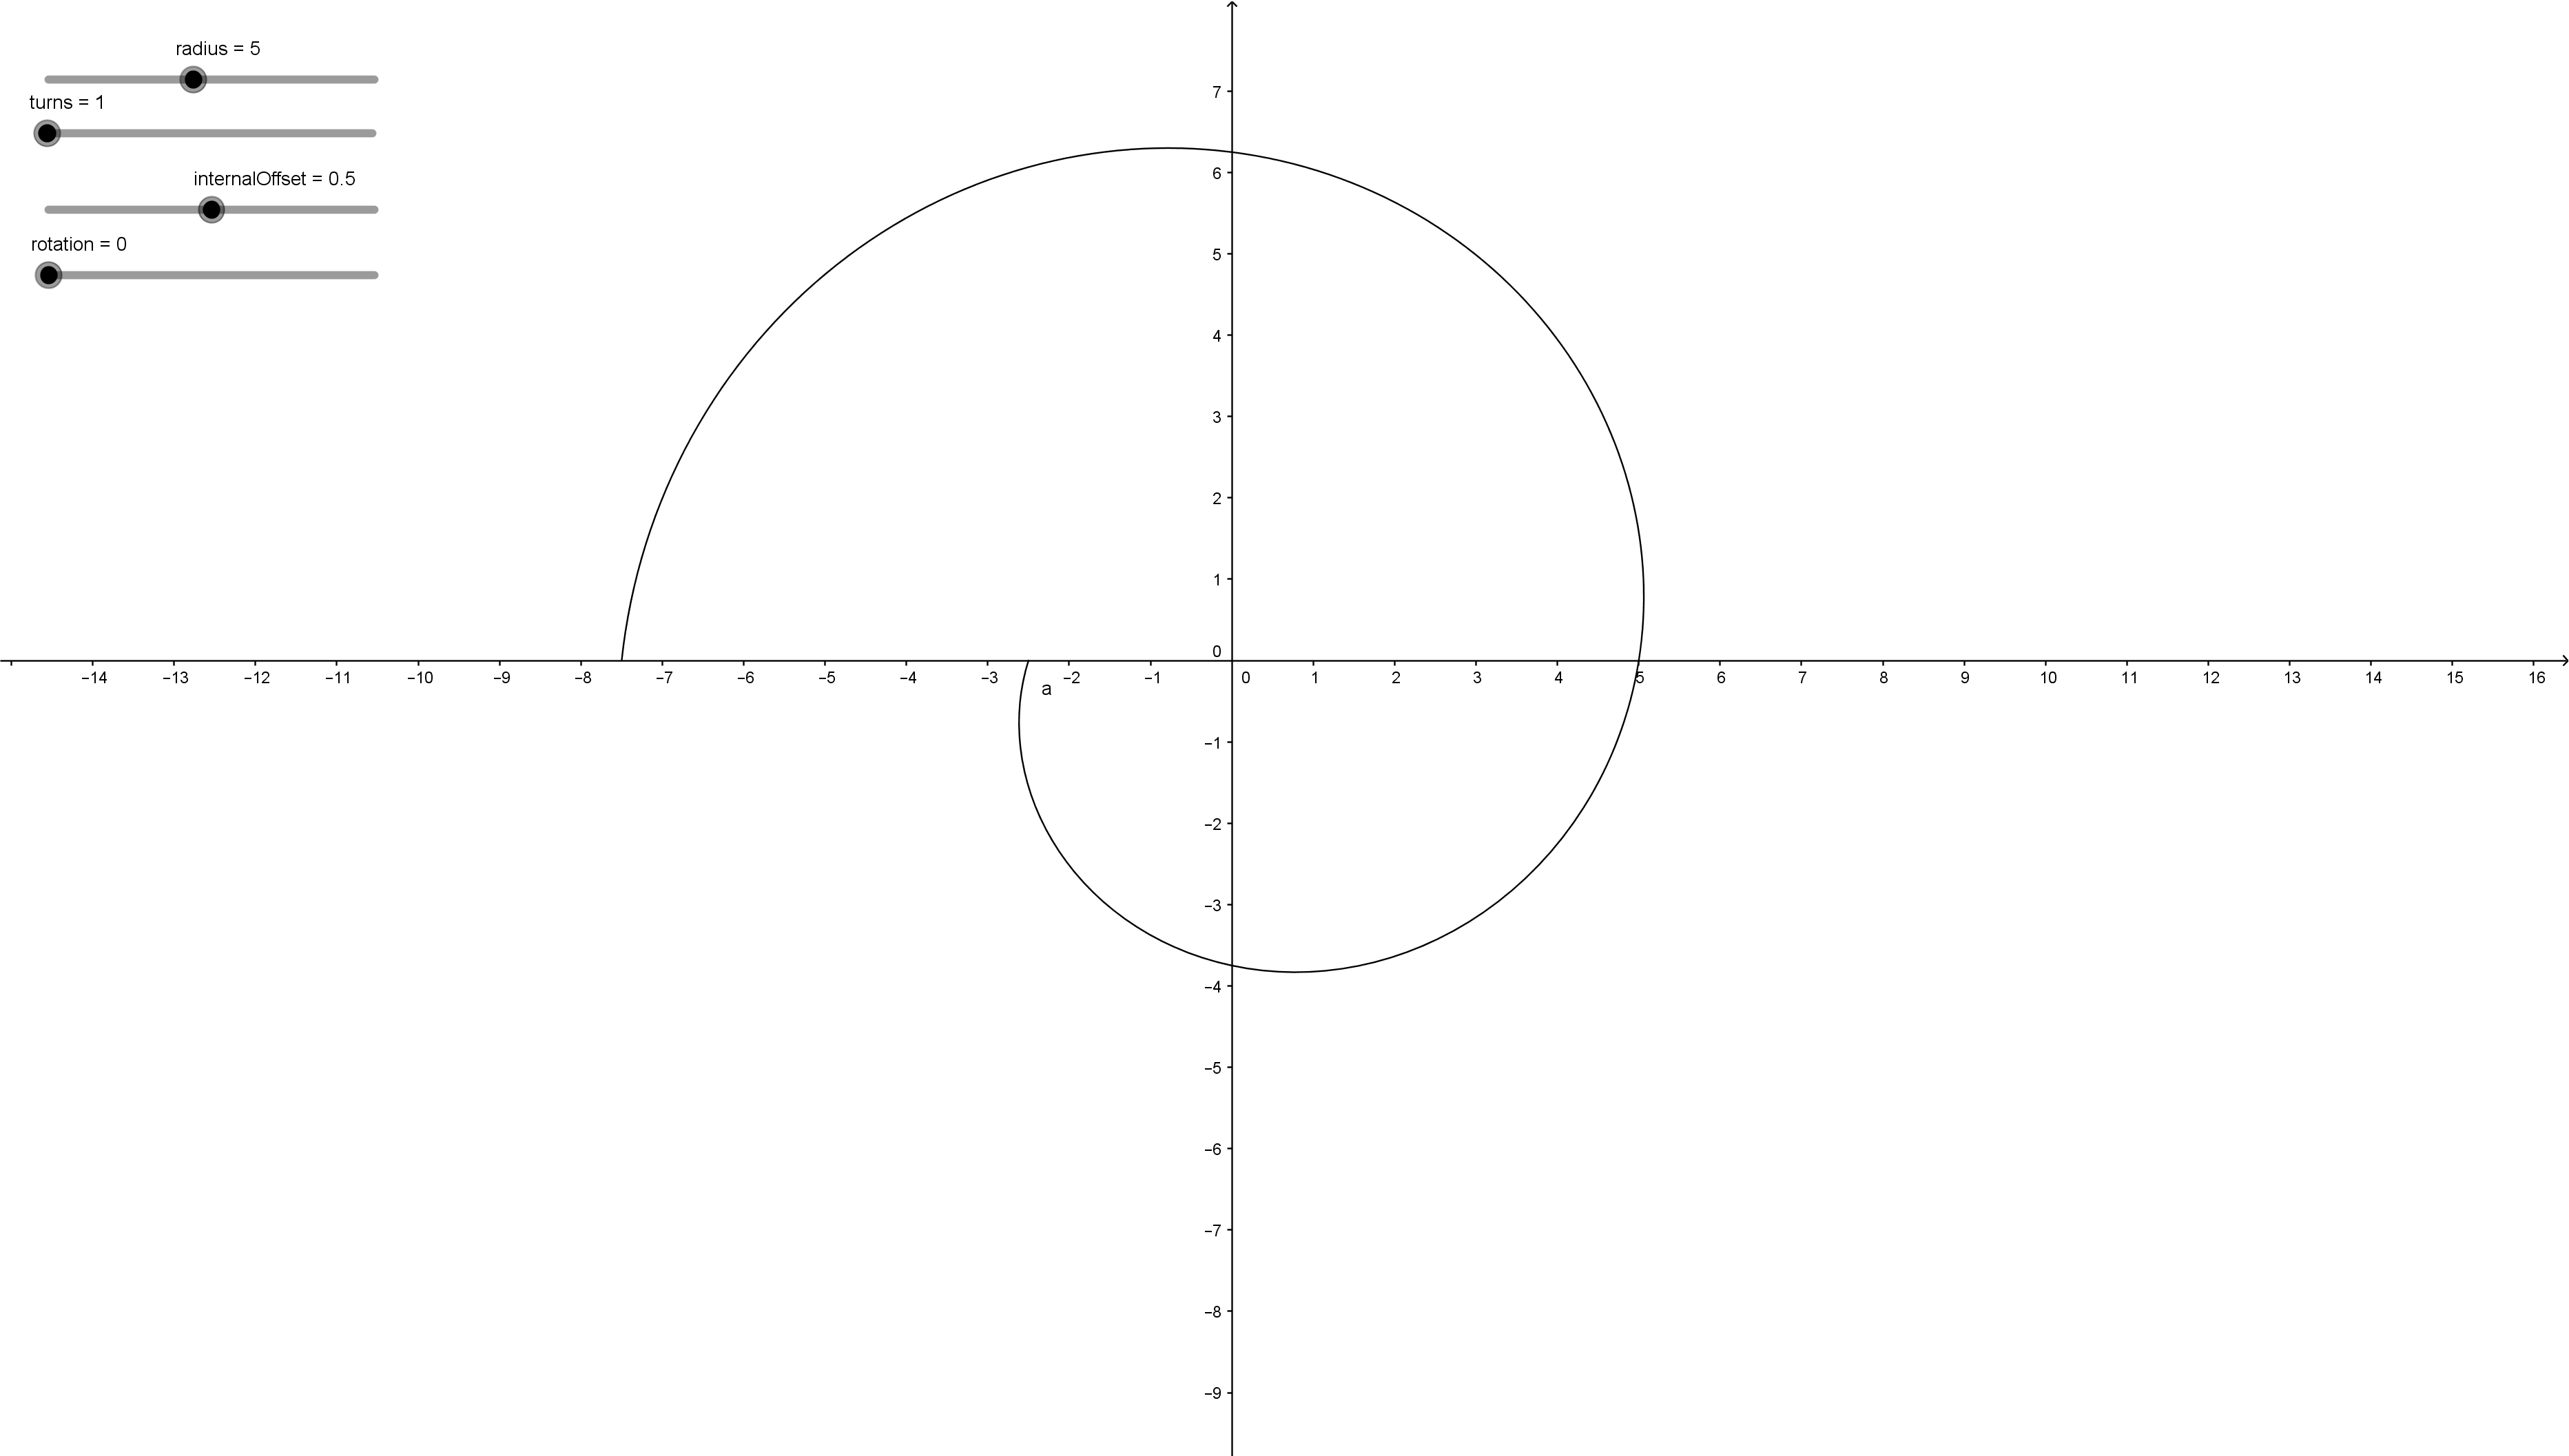
\includegraphics[scale=0.2,trim={10cm 4.65cm 11.3cm 3.0cm},clip]{img/spiral/5internaloffset}
&
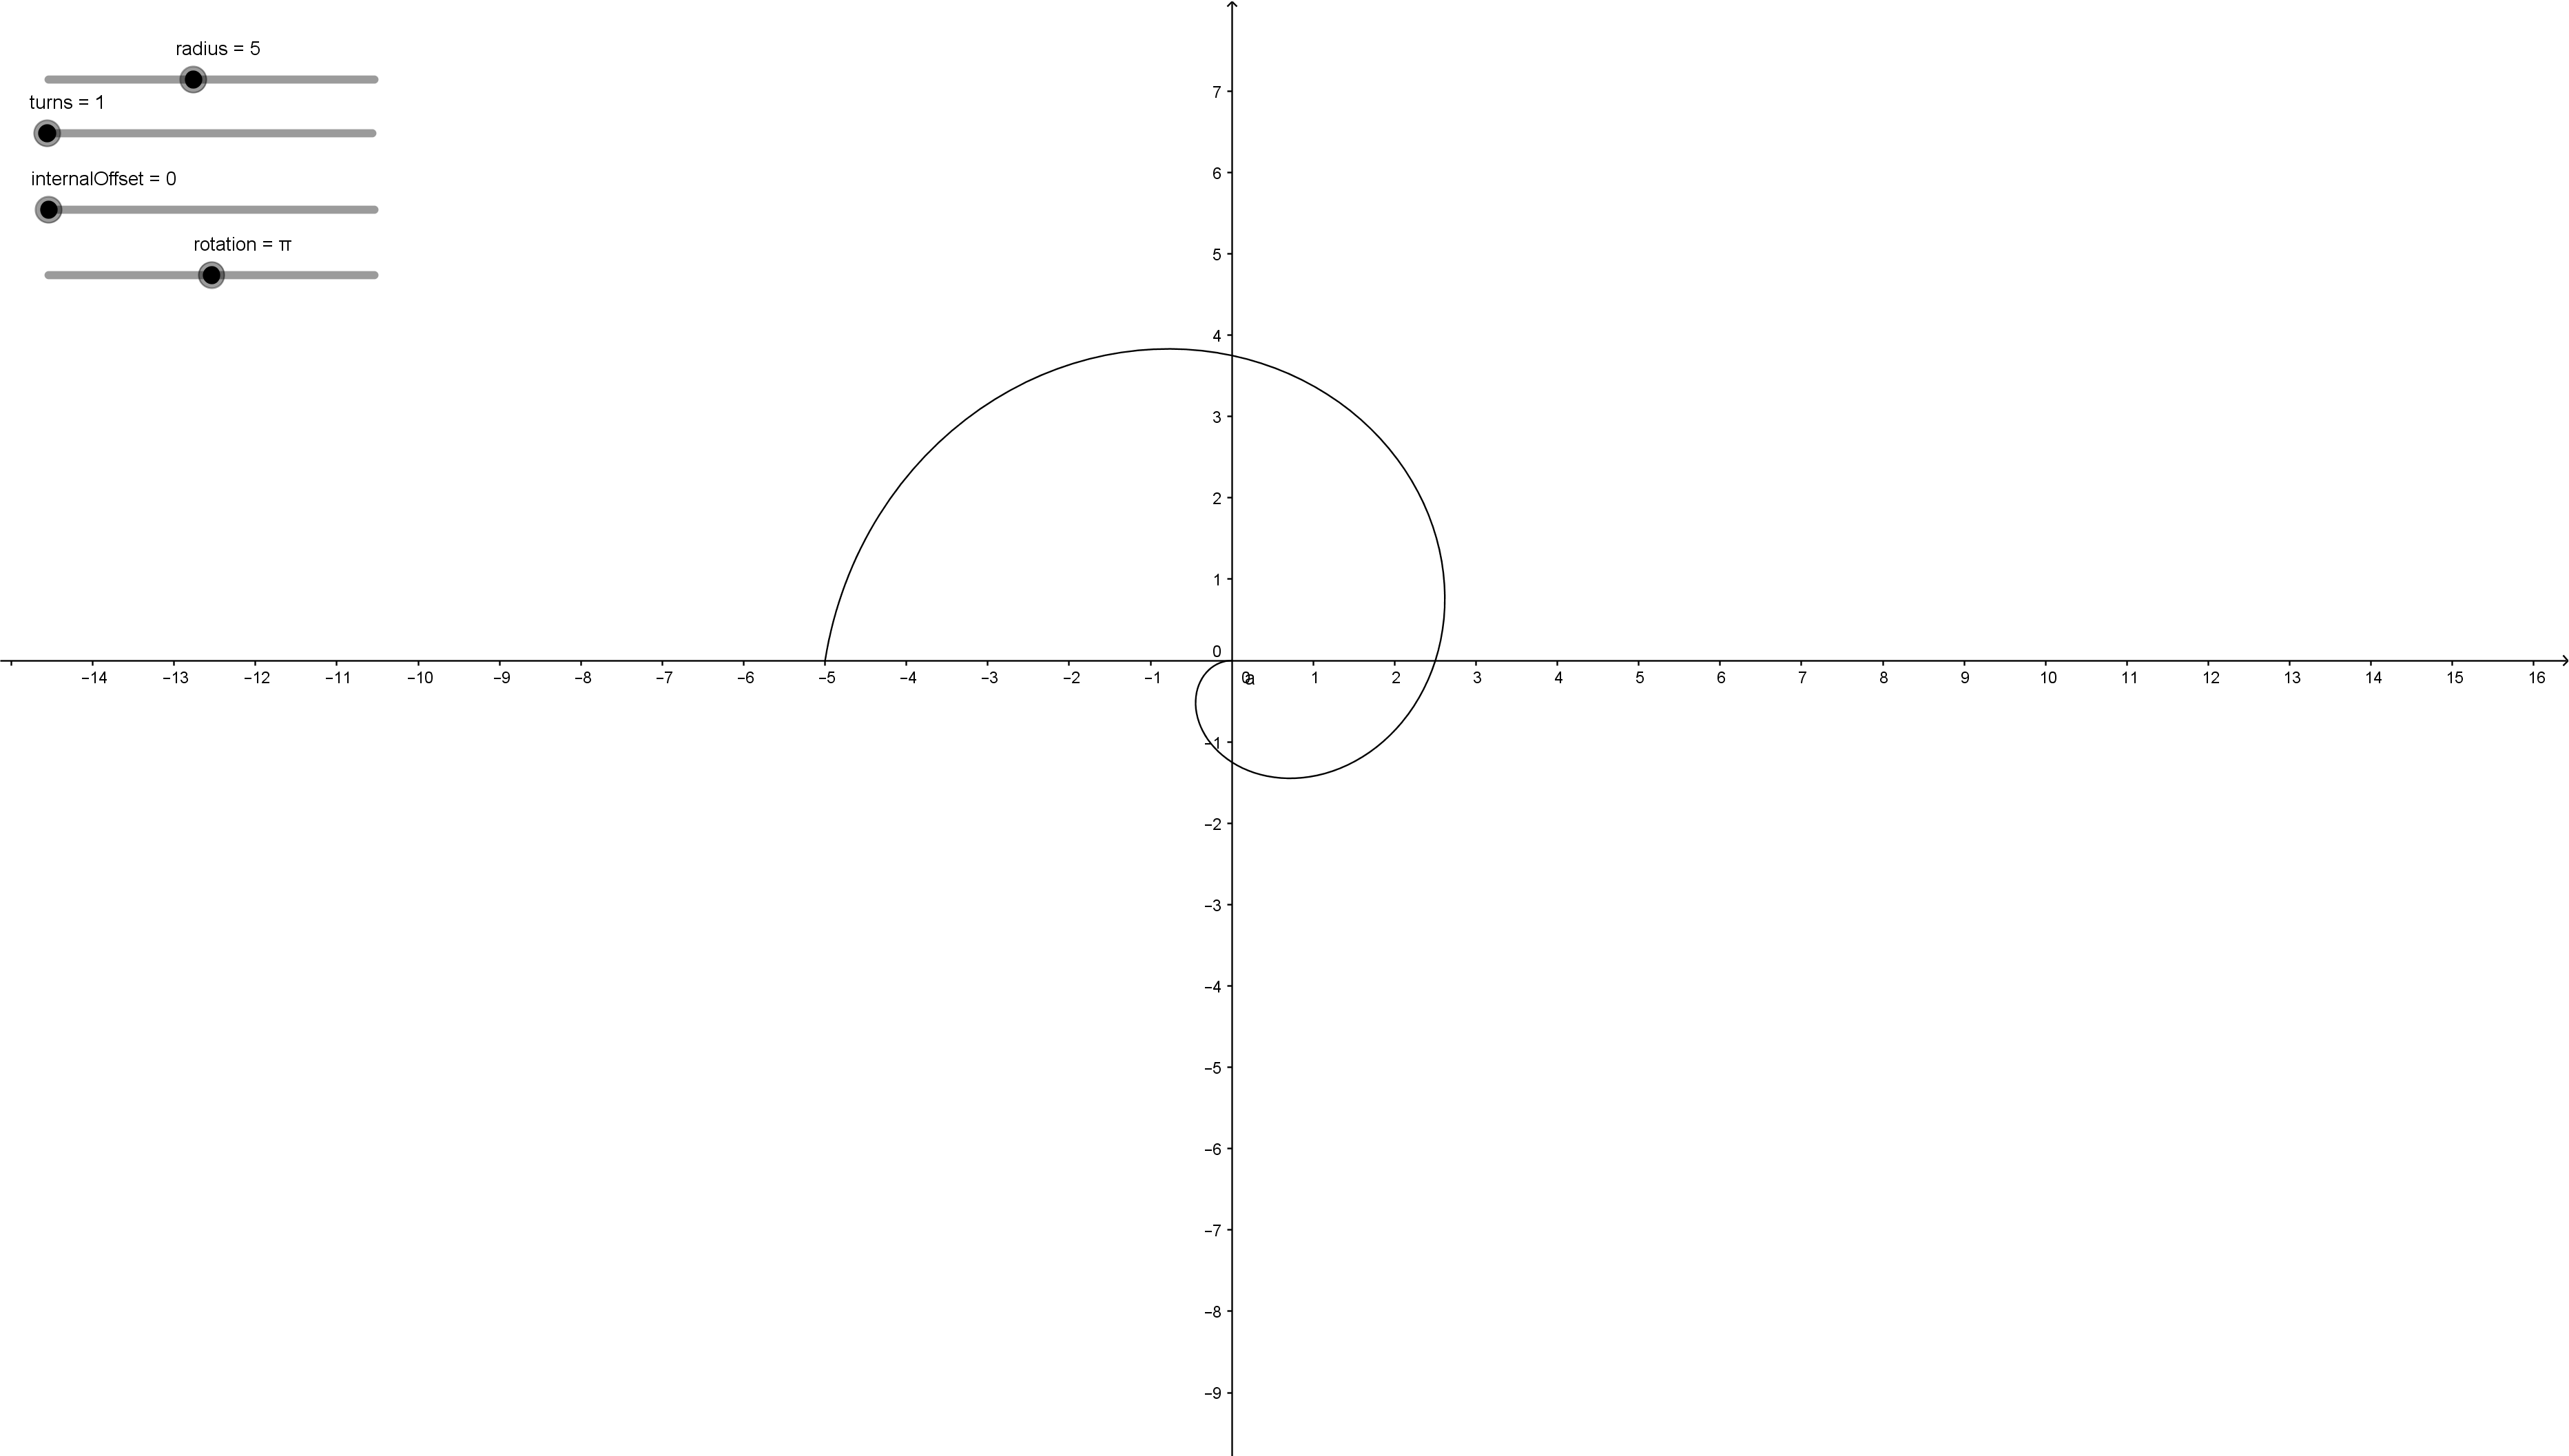
\includegraphics[scale=0.2,trim={10cm 4.65cm 11.3cm 3.0cm},clip]{img/spiral/pioffset}
\\
\hline
R (Radius) & $5$ & $5$ & $5$ & $5$ \\
\hline
$\tau$ (Spiral Turns) & $1$ & $5$ & $1$ & $1$ \\
\hline
$\phi$ (Rotation) & $0$ & $0$ & $0$ & $\pi$ \\
\hline
$\psi$ ($t$ Offset) & $0$ & $0$ & $0.5$ & $0$ \\
\hline
\end{tabular}
\caption{Demonstrates the consequence of different parameters for the spiral curve.}
\label{fig-spiralparam}
\end{figure}

We sample along the spiral by incrementing $t$ discretely from 0 to 1 given a certain number of samples. To achieve this we replace the form of $\theta$ by $\theta_i = \frac{i + \frac{\psi}{\tau}}{n}$ where $n$ is the number of samples we do. We end up with an algorithm that sums up irradiance like so:

$$\mathbf{p_i} = \mathbf{x} + \mathbf{v_i}$$
$$\overline{\omega_i} = | reconstruct(\mathbf{p_i}) - \mathbf{X} |$$
$$B(\mathbf{x}) = K_d \frac{2\pi}{m} \sum_{i = 0}^{n} B(\mathbf{p_i}) (\overline{n_X} \cdot \overline{\omega_i})$$

Where $X$ is the spatial point reconstructed from the screen-space tap $\mathbf{x}$ (our current gathering point,) $reconstruct()$ is a function that reconstructs the spatial point from the screen-space tap $\mathbf{p_i}$ and $m$ is the number of "accepted" sample taps. We discard all sample taps that are not on the hemisphere of $\mathbf{X}$, and the ones which extend beyond screen-space.

We need one final piece, and that is to determine the total number of spiral turns. For that we use the array defined in \cite{deep-g-buffer}. It is important that we fit the number of spiral turns to the number of sample taps, since not doing so can cause the taps to become "synched" from one turn to the next, meaning the spread is minimised. We tap both layers of the G-buffer at the same sample point positions in screen-space.

The final result of this method appears grainy as seen in figure \ref{fig-noise}, since we have traded off structural bias for more randomised noise. To alleviate this we will applya gaussian filter over the radiosity result. This filter is described in section \ref{section-gauss}.

\begin{figure}[!ht]
  	\centering
  	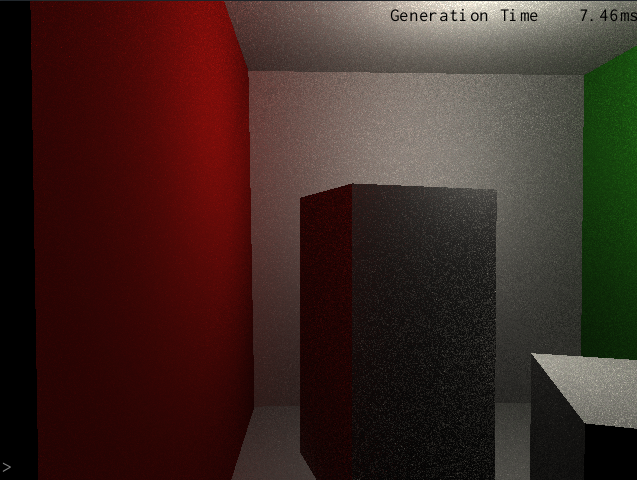
\includegraphics[width=0.8\textwidth]{img/noise}
    \caption{Unfiltered Radiosity result showing high level of random noise}
    \label{fig-noise}
\end{figure}

\section{SSAO}
SSAO or Screen-Space Ambient Occlusion is a way to evaluate the occlusion of ambient light for a given fragment, based on information available in the G-buffer. We use the alchemy AO method for this purpose:\cite{VV11AlchemyAO}

$$AO(\mathbf{X}) \approx max \left( 0 , 1 - \frac{2 \sigma}{s} \sum_{i = 1}^{s} \frac{max(0,\overline{v_i} \cdot \overline{n} + \mathbf{X_z} \beta)}{\mathbf{v}_i \cdot \mathbf{v}_i + \epsilon} \right) ^K$$

This function has a lower value the more geometry "covers" its hemisphere. The parameters to it are as follows:
$s$ is the number of samples.
$\sigma$ controls magnitude. The higher it is, the less it takes for geometry to count towards the obscurance of $\mathbf{X}$.
$\beta$ is used to reduce self-shadowing, but leaving it too high can cause lack of contributions.

We divide by the dot product of the $\mathbf{v}_i$ vector by itself in order to get some scaling with the size of the scene.

\section{Filtering}
The spiral for each individual pixel can be rotated by any value within $[0;2\pi]$, and only does $20\pm10$ samples per buffer layer, within a radius that spans tens of thousands of pixels. As such, there's a high amount of high-level noise, resulting in a grainy image with potentially big contrasts from pixel to pixel. Therefore, we need a filtering method which will level out the radiosity and AO to more smooth results across surfaces. To this end we will employ a traditional gaussian blur filter, with some modifications to improve on running time and avoid surfaces "bleeding" in to each other.

\subsection{Gaussian Filtering}
\label{section-gauss}
We employ a filter by looping through all pixels in our buffer, and for each pixel we wish to even its intensity out with its immediate neighbours. We do this in a radius around our center pixel, which we will denote by $R$. We denote our center pixel (that is to say the pixel for which we are currently applying the filter) by $P_c$ and the pixel at position $(x,y)$ in relation to $P_c$ as $P(x,y)$.
The Gaussian Filter is a filtering method that aims to average out neighbouring pixels according to their distances to each other as an argument to the Gaussian Function, also known as the bell curve or the normal distribution. In general terms, the Gaussian Function, $G(x)$ is defined as follows,

$$G(x) = \frac{1}{\sigma \sqrt{2\pi}} e ^ {-\frac{(x - \mu)^2}{2\sigma^2}}$$

In which $\sigma$ denotes the standard deviation and $\mu$ the mean. In the traditional normal distribution with $\sigma = 1$ and $\mu = 0$, $68\%$ of the area under the graph of the function will be within the interval $[-1;1]$. A plot of this function is seen in figure \ref{fig-gauss}.

\begin{figure}[!ht]
  	\centering
  	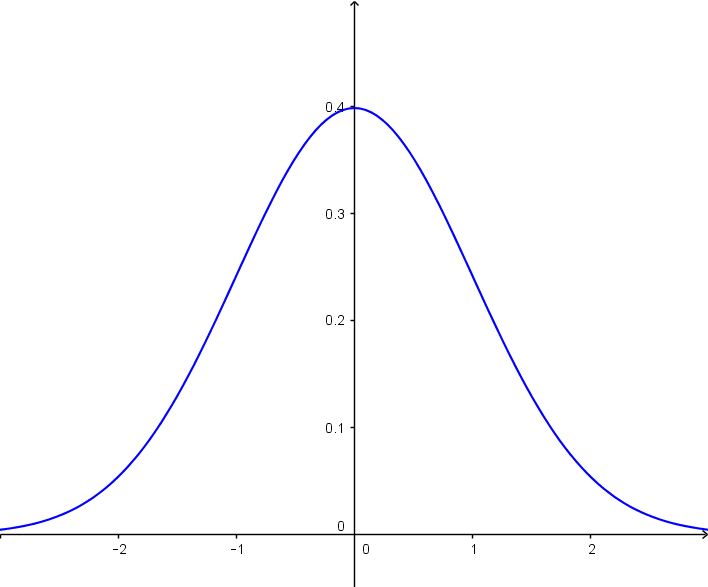
\includegraphics[width=0.8\textwidth]{img/gauss}
    \caption{Gaussian Function plot with $\mu = 1$ and $\sigma = 1$}
    \label{fig-gauss}
\end{figure}

This particular function is advantageous to averaging out colour values across a surface, since it tends towards zero the farther away we get from our central point, and it does so on a smooth curve. An alternative method in which we took the naïve average over a radius would create blocky artefacts, since values at the edge would count the same as values closer to our central point.

\subsubsection{Image Filter}
We wish to fit the Gaussian Function to filter our radiosity and AO outputs, and a simple way to do so is to loop over all neighbouring pixels within radius $R$, and weigh their sampled values by the Gaussian of their distance to $P_c$. If we consider $B\prime(P_c)$ the filtered radiosity output for our point $P_c$, then we would find that value like so:

$$B\prime(P_c) = \frac{1}{W} \sum_{i = -R}^{R} \sum_{j = -R}^{R} G(|(i,j)|) \cdot B(P(i,j))$$
$$W = \sum_{i = -R}^{R} \sum_{j = -R}^{R} G(|(i,j)|)$$

We divide by the sum of all Gaussian weight values, since we're essentially doing a weighted average with the Gaussian Function as our weight.

Finally, we need to pick out the proper values of $\mu$ and $\sigma$. If we consider the distance from our central point to as the argument to $G(x)$, then we set $\mu = 0$. This means that our central point, $x = 0$, will have the highest weight. The standard deviation $\sigma$ will have to be picked such that our farthest point, $R$ is very close to zero. It is typical to say that this happens after three standard deviations, and as such we get $\sigma = \frac{R}{3}$. Figure \ref{fig-gauss-applied} demonstrates the application of this algorithm to a 11x11 image with a single white pixel in the center. The color of the center pixel has been spread across the other pixels according to a Gaussian distribution.

\begin{figure}[!ht]
  \centering
    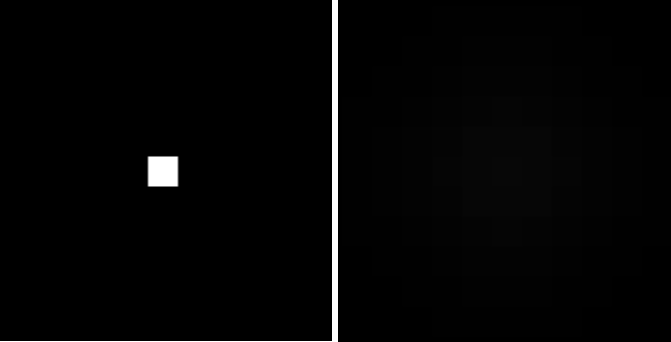
\includegraphics[width=0.8\textwidth]{img/gauss-pixel}
    \caption{The Gaussian filter applied to an 11x11 black square with a single white pixel. Right hand side is after the 									filter has been applied}
    \label{fig-gauss-applied}
\end{figure}

One quick performance improvement is to remove the factor $\frac{1}{\sigma \sqrt{2\pi}}$ from the Gaussian function since it is eliminated from the equation when we divide by $W$. As such we are left with the following function to replace $G(x)$

$$\gamma(x) = e ^ {-\frac{(x - \mu)^2}{2\sigma^2}}$$

\subsubsection{Modifications}
Running a filter over a full rectangle for every pixel would have a complexity of $O(n^2)$, where $n=2R + 1$. This is infeasible for large radii. Additionally, we want to employ some method of avoiding surfaces "bleeding" into each other. One way to achieve the latter to employ a bilateral filter\cite{bilat}, in which some function value of difference in intensity between two pixels is added as a factor to the weight of a pixel. One problem with this approach, however, is that it our final radiosity and AO results both have big differences between pixels on the same surface. As such, we will in stead employ a function of the depth difference between the two. We would like to also use the normal in some capacity, to accommodate adjacent but differently facing surfaces, but the results don't seem to be worth the extra loss in performance. In other words we add the term $Z_{factor}(x,y) = (1 - ||Z_{xy} - Z_{P_c}||)$ to the weight of a given sample point.

In terms of performance, we will turn the filter into a 2-pass one in stead of the original 1-pass. That is to say, in stead of polynomial complexity, we wish to make it linear. Essentially we wish to swap the original equation for our Gaussian weight with the following:

$$B\prime_{1st}(P_{c}) = \frac{1}{W} \sum_{i = -R}^{R} \gamma(i) Z_{factor} B(P(i,0))$$
$$B\prime(P_{c}) = \frac{1}{W} \sum_{i = -R}^{R} \gamma(i) Z_{factor} (x,y) B\prime_{1st}(P(0,i))$$
$$W = \sum_{i = -R}^{R} Z_{factor}(x,y) \gamma(i)$$

This filter runs in O(n) time and is thus much more suitable for averaging out large surfaces.  It also removes the use of length as an argument to the gaussian function, since we can now just use the value of $i$ as the argument.